% !TEX program = xelatex
\documentclass[a4paper]{report}

\usepackage{amssymb}
\usepackage{amsmath}
\usepackage{amsthm}
\usepackage{CJKutf8}
\usepackage{enumerate}
\usepackage{fancyhdr}
\usepackage{geometry}
\usepackage{graphicx}
\usepackage{indentfirst}
\usepackage{latexsym}
\usepackage{mathrsfs}
\usepackage{textcomp}
\usepackage{url}
%\usepackage{unicode-math}
\usepackage{flafter}
\usepackage{booktabs, longtable}
\usepackage{pxfonts}

\usepackage[perpage,symbol]{footmisc}
\setfnsymbol{wiley}
\usepackage{hypbmsec}
\usepackage{dsfont}
\usepackage{graphicx}
\usepackage{subfigure}
\usepackage{listings}
\usepackage{xcolor}
\usepackage[algo2e,lined,boxed,linesnumbered]{algorithm2e}
\usepackage{layout}
\usepackage{tikz}
%\usepackage{cite}

\newcommand{\tabincell}[2]{\begin{tabular}{@{}#1@{}}#2\end{tabular}}
\newcommand{\Dim}{\mathrm{D}}
\newcommand{\cond}{\mathrm{cond}}
\newcommand{\ebold}{{\mathbf{e}}}
\newcommand{\ibold}{\mathbf{i}}
\newcommand{\jbold}{\mathbf{j}}
\newcommand{\avg}[1]{\left\langle #1 \right\rangle}
\newcommand{\dif}{\mathrm{d}}
\newcommand{\Lapl}{{\mathbf{L}}}
%==============================================================
%==============================================================
\begin{document}
	\begin{CJK*}{UTF8}{gkai}
		\CJKindent
 
 %------------中文设置--------------------------
 \makeatletter %将文献引用作为上标出现,增加括号,
 \def\@cite#1#2{\textsuperscript{[{#1\if@tempswa , #2\fi}]}}
 \makeatother
 \newtheorem{thm}{{定理}}[chapter]
 \newtheorem{lem}[thm]{{引理}}
 \newtheorem{defn}[thm]{{定义}}
 \newtheorem{prop}[thm]{{命题}}
 \newtheorem{cor}[thm]{{推论}}
 \newtheorem{exm}{{例}}[chapter]
 \newtheorem{rem}[exm]{{注}}
 \newtheorem*{pro}{证明}
 %\newtheorem{prop}{{命题}}[chapter]
 
 \renewcommand{\bibname}{\centerline{参考文献}}
 \renewcommand{\tablename}{表}
 %\renewcommand{\captionlabeldelim}{\quad}
 %===================Image settings========================%
 \renewcommand{\figurename}{图}
 

 \title{三维界面追踪的线性MARS方法}
 \author{潘瑛芝}
 \date{}
 \maketitle
 
  %\newpage
  %序言
  %\input{preface} % 请根据需要取舍。
  %中文摘要
  %% 中文摘要
\chapter*{\centerline{摘\quad 要}}
\chaptermark{摘要}
\addcontentsline{toc}{chapter}{摘要}

\vspace{1em}
多相流在许多的重要领域发挥着关键作用,一直以来都是科学研究的热门课题,而界面追踪问题作为其最基本和最重要的子问题之一,迄今为止已经发展了许多的方法.现有的方法回避复杂的拓扑问题,致力于将几何拓扑问题转换成求解数值微分方程,不管是在精度上还是在流相的拓扑变化处理上都有着一定的局限性.而MARS理论和高阶数值方法用几何拓扑工具来处理界面追踪问题,最大程度地保留了流相的界面特征.本文将MARS方法从二维情况推广到了三维的情况,作为开创性的工作,本文限制在流函数是同胚映射的简单情况下.文章首先简要介绍了MARS理论的基本内容,并在此基础上定义了三维殷空间作为连续介质流相的数学模型.然后,文章采用了2-复形来表示流相边界,提出了一个三维空间上的界面追踪法linear MARS,并且通过误差分析证明了其二阶精度.最后,进行了三个经典的数值实验,分别将不同的流场作用在三维球上,展示了linear MARS方法的测试结果以及其二阶精度.

\vspace{1em}

关键词:界面追踪;MARS理论;单纯复形;布尔代数;殷空间

  %英文摘要
  %% 英文摘要
\chapter*{\centerline{Abstract}}
\chaptermark{Abstract}
\addcontentsline{toc}{chapter}{Abstract}

\vspace{1em}
The study of multiphase flows plays a key role in many important fields and has always been a hot topic in scientific research. Interface tracking (IT) is a fundamental problem in the study of multiphase flows. Many IT methods have been developed for accurate and efficient numerically simulate of multiphase flows. Existing methods avoid complex topological problems by converting geometric topological problems into numerical differential equations. However, there are some limitations in accuracy and modeling topological changes of the flow phase. The MARS method and the high-order numerical method use geometric and topological tools to solve the IT problems while retaining the interface characteristics of the flow phase to the greatest extent. In this paper, the MARS method is extended from the 2D case to the 3D case. As a seminal work, we restrict ourselves to the simple case of the flow map being a homeomorphism to avoid tackling   topological changes. Starting with the foundation of the MARS framework and the defined Yin space as a modeling space of 3D phases, we use 2-simplicial complex to represent the boundary of the flow phase, and develop linear MARS, an interface tracking method in 3D.  Finally, three classical numerical experiments are carried out to show the test results and the second-order accuracy of the linear MARS method.


\vspace{1em}

\textbf{Keywords:}~~interface tracking; MARS theory; simplicial complex; Boolean algebra; Yin space


%==============================================================
%这部分不需要自己修改。


  %插图和附表清单
  %\listoffigures
  %\chaptermark{图目录}
  %\addcontentsline{toc}{chapter}{图目录}
  %\listoftables
  %\chaptermark{表目录}
  %\addcontentsline{toc}{chapter}{表目录}
  %术语表
  % \printnomenclature
  % \chaptermark{术语表}
  %目次页
  %\tableofcontents
  %\addtocontents{toc}{\protect\chaptermark{目录}}
  %\addtocontents{toc}{\protect\contentsline {chapter}{\protect\makebox[\linewidth]{目录\hfill}\vspace{-2em}}{}}
  %\mainmatter

%==============================================================

 
\chapter{绪论}
\label{chap_int}
\section{选题背景与意义}
多相流的研究在许多现代科学技术的发展上都起到了一定的指导作用,
其在水利工程、国防安全、航空航天、现代医学、核能工程等各个重要领域都有着举足轻重的地位.
科技的发展和时代的进步同样也推动着多相流的研究不断进步,使得其日益精细化与复杂化.
其中多相流的数值模拟更是凭借着自由灵活、可重复实验、耗费少等优点,
已经成功替代了许多费用昂贵、难以实现的实验,
例如:油藏量的勘测,泄洪闸室的性能研究等,图\eqref{fig:example}.
多相流的数值模拟不仅能够极大地降低科研的成本,还大大缩短了一些科学项目的研究周期.

 \begin{figure}[htbp]
 	\label{fig:example}
	\centering
	\subfigure[多相流数值模拟勘测油储量]{
		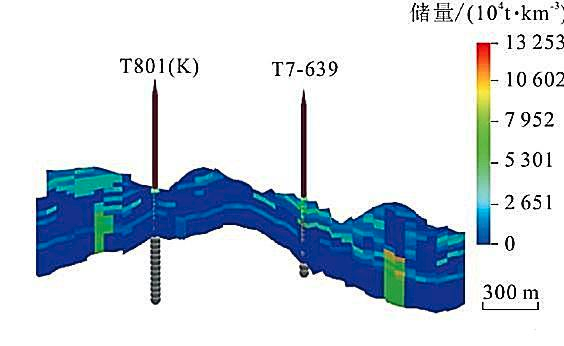
\includegraphics[width=0.45\linewidth]{images/aaa}
	}
	\hfill
	\subfigure[多相流数值模拟泄洪闸室的水流速度]{
		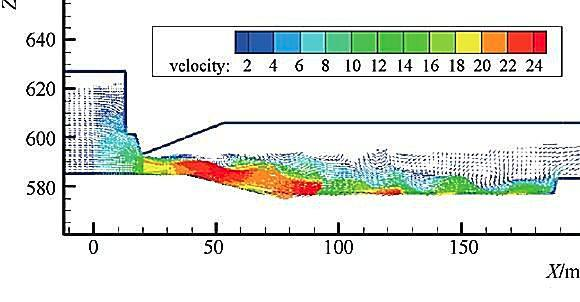
\includegraphics[width=0.45\linewidth]{images/bbb}
	}
\caption[多相流数值模拟的例子]{多相流数值模拟的例子}
\end{figure}

在多相流的数值模拟过程中,界面追踪的精度很大程度上影响了其保真度.
首先,流体自身的计算精度必然受界面追踪的误差所影响.
其次,流体曲率估算的误差与界面追踪的误差存在着密切的关系\cite{zhang17:_hfes}.
在多相流的问题研究中,有些流相的表面张力不可忽略,此时的曲率估计若不够准确,
界面上有可能产生伪波,界面因此失稳破碎,最终的计算结果也背离了物理规律\cite{denner14:comparative,francois06:balanced_force,lafaurie94:modeling}.
可见,界面追踪问题是多相流的研究中最基本且最重要的子问题之一.
然而,在许多多相流的研究中,流体界面会在几何上产生巨大的形变,
流相也可能有着潜在的拓扑变化,故界面追踪问题也因此面临着巨大的考验和挑战.




\section{现有界面追踪方法介绍}
在过去的几十年中,已经发展了许多的界面追踪法,
其中应用最广泛的三种方法分别是:
level set(LS)方法\cite{osher88:_front_propag_curvat_speed}、volume of fluids(VOF)方法\cite{Hirt.Nichols_1981_volume}
以及front tracking(FT)方法\cite{tryggvason01:_front_track_method_comput_multip_flow,unverdi92:front_tracking}.
在上述的这些方法基础上,近些年来还衍生出了一些变体方法、混合方法和自适应方法
\cite{ahn07:_multi,ahn09:_adapt,chenadec13,li03:_fixed_part_i,
diwakar09:_quadr_splin_based_inter_quasi,dyadechko05:_momen,
dyadechko08:_recon,enright02:_hybrid_partic_level_set_method,ginzburg01:_two_vof,
harvie00:_new_volum_fluid_advec_algor,
lopez04:_volum_fluid_method_based_multid,scardovelli03,
sussman99,sussman03SpectralLevelSet,sussman00:_coupl_level_set_volum_fluid,
wang12HLSVC,zhang13:VOFadvection,zhang08:_new_inter_track_method}.

\subsection{Level Set (LS)方法}
LS方法又称等值面函数法,是多相流界面追踪数值模拟的一种比较流行的方法且在许多方面都得到了应用.
LS方法最初是在1988年由美国计算数学家Stanley Osher等人提出.
LS方法的核心思想是在流场中设定一个等值面函数$\varphi(x,t)$且满足:
\begin{equation}\label{eq:LS}
\varphi_t+\mathbf{u}\cdot\bigtriangledown \varphi=0,
\end{equation}
等值面函数$\varphi$在流相交界面上的值是$0$.
在任意时刻,求解控制方程\eqref{eq:LS},得出其零等值面,便可定位流相的交界面.
LS方法不需要显式地表示界面,这一特点提高了其追踪复杂的界面的能力,
能够更容易地处理发生拓扑结构变化的情形.
由于在新的时间点,式\eqref{eq:LS}的解不再是新界面的等值面函数,
因此需要对LS函数重新初始化.
在经过有限的时间步长之后,其梯度可能变得平缓或剧烈,等值线也会因此出现聚合或者拉伸的情形,
这将使其不再继续保持距离函数的特性.
为了优化LS算法,Osher等人又对LS重新初始化的方法进行了深入研究.
考虑到边界只在某一局部区域内改变位置,故可以仅在该较小区域上求解LS方程,
这个方法被称为快速局部LS方法.
快速局部 LS方法大大加快了界面追踪的计算效率,同时也缩小了计算的存储量,提高了其实用性.
LS方法现如今已应用于多个行业,用来解决曲面重建、图像处理、最优化等各类问题.

\subsection{Volume of Fluids (VOF) 方法}
1981年,Hirts和Nichols在论文中首次提出了VOF方法,
该论文对于溃坝和涌浪的界面追踪问题进行了数值模拟.
VOF方法自提出以来,其基本思想受到广泛重视,
尤其是为输运界面的重构提供了开创性的思路.

VOF针对被追踪的流相M定义一个变量标记函数
\begin{equation}\label{bilevel}
f(\mathbf{x},t):=
\left\{\begin{array}{l}
1  \qquad \text{若}(\mathbf{x},t)\text{处含有流相介质},\\[0.2cm]
0  \qquad \text{若}(\mathbf{x},t)\text{处无流相介质}.\\[0.1cm]
	\end{array}\right.
	\end{equation}
对每一个控制体$\mathcal{C}_{i,j}$定义容积比
\begin{equation}
f_{i,j}(t) :=\int_{\mathcal{C}_{i,j}} \frac{1}{\|\mathcal{C}_{i,j}\|}f(\mathbf{x},t).
\end{equation}
在每一个时间步中,VOF方法可以再成两小步:
重建步根据边界控制体中的容积比和速度法向,
在边界单元中确定一条切线或多项式曲线,以此来近似流相的显式边界的位置,
用此结果得到的边界作为边界条件;
对流步则根据重建步得到的边界条件以及给定的流场条件
来重新计算获得每个控制体在该时间步内所产生的容积比的变化.
其中,许多的VOF方法以标量守恒来作为其理论依据,
\begin{equation*}
\frac{\partial f}{\partial t}+\nabla \cdot (f\mathbf{u})=0.
\end{equation*}
VOF保持了体积守恒,方便计算复杂的界面变化过程,
如波浪的翻卷、破碎、溶并等,已用于许多实际的模拟计算中.

\subsection{Front Tracking (FT)方法}
与VOF方法和LS方法相比,
FT方法则是通过完全显式的形式将界面用一个单独的非结构化的网格表示.
在二维情况中,FT方法将示踪点用直线相连接来近似边界;
在三维情况中,FT方法用三角平面组成的曲面来近似边界.
网格通过流场输送时,FT方法追踪每一个时间步示踪点的位置,
在进行追踪的过程中,网格界面在流场的作用下会产生位移并且不断地变形,
因此追踪过程中需要对网格进行不断地重构.
FT方法在追踪流相界面时,
其用于表示界面的示踪点的相邻两点之间的距离$h_L$能够远远小于流体内部尺度$h$,
这一特性让FT方法能够精确的锁定流相发生拓扑变化的时间点和位置\cite{brochu09},
使得它拥有了隐式方法所不具备的突出优势.

\section{现有界面追踪方法的局限性分析}
现有的界面追踪方法在许多方面都取得了重要的成就,
但依然存在着一些局限性.
这些局限性使得现有方法难有进展,更限制了多相流研究的发展.

第一,现有方法的计算精度往往不够高.

首先,在流场涡量强、界面变形大的多相流数值模拟中,
LS方法和FT方法界面追踪的误差大且难以保持体积守恒.
其次,当运动界面存在尖点(在边界上$C^1$不连续的点)时,
LS方法和VOF方法将难以保持其形状特征,它们会使得尖点附近趋于平滑.
即使在网格很密的情况下,这一局限性也无法得到有效的改善.
当多相流中包含三个或三个以上流相时,这样的尖点必然存在,
这意味着LS方法和VOF方法的精度会随着尖点的出现而进一步下降.
由文献\cite{zhang13:VOFadvection,zhang14:iPAM}得知,现有VOF方法以及FT方法最高只有二阶精度,
又由于尖点引起的精度下降等原因,很多二阶精度的方法实际上都没有达到二阶精度.
最后,在曲率估算方面,现有的研究\cite{cummins05,denner14:comparative}结果表明,
VOF+HF方法\cite{helmsen97,sussman03}是最精确的方法之一,
而此方法的曲率估计误差存在下界,下界会随着方法收敛阶的增加而减小.
其中对于二阶方法来说,曲率估计误差$\epsilon_{\kappa}$和
界面追踪误差$\epsilon_p$之间满足$\epsilon_{\kappa} \sim O(\sqrt{\epsilon_p})$的关系\cite{zhang17:_hfes}.
这就是说,界面追踪的有效数字有一半会丢失在曲率估计的时候,若界面追踪的精度不够高,
那对于实现曲率的准确估计就更加困难了.

第二,现有方法对于流体的拓扑变化处理无力.

LS和VOF方法将几何拓扑问题转化成了求解数值偏微分方程问题,
无须对流相的拓扑变化进行特殊处理,
这种特性虽然从某种程度上简化了问题,
但在界面追踪中回避几何拓扑的方式从长远发展上来看是治标不治本的.
从物理的角度而言,在界面追踪的过程中,当流相发生拓扑变化时,
具体的变化细节应根据流相的物理性质来考虑,
而不是简单的“自动化”就能进行统一处理的,
LS方法和VOF方法很难将流相的物理性质高精度地反应到界面追踪的算法中\cite{zhang14:iPAM}.
此外,当流速场足够连续时,相应的流函数应是同胚的,
而LS方法和VOF方法在追踪过程中可能存在改变流相拓扑的情况,
这和流函数是同胚映射的事实相违背.
最后,现有方法在处理流相的拓扑变化时可能产生较大的误差.
例如,当VOF方法在处理尺度小于控制体边长$h$的界面合并时,
每一个产生拓扑变化的控制体将造成$O(h^{\textup{D}})$的误差(D是计算域维数).
已知边界的控制体个数是$O(1/h^{\textup{D-1}})$,时间步数是$O(1/h)$,
因此当多相流的拓扑变化过于频繁时,
时间和空间上的误差累计可能会使得VOF方法的界面追踪结果不收敛.

第三,显式的界面追踪方法缺乏系统的理论分析体系.

LS方法的理论分析体系相对较完备\cite{falcone14,giga06,sethian97},
不论是在解的唯一性\cite{chen91,evans91,giga92}、稳定性,
还是对于解的收敛性\cite{barles91,crandall96,decknlnick00,falcone98,falcone01,walkington96}上都有相关的证明.
与LS方法相比,关于显式FT方法的理论分析则在文献中很少见,
这可能是因为FT方法常常需要一些不严格的假定,
在拓扑变化的处理上一般针对特定条件及特殊应用来进行算法设计.
由此可见,FT方法不具有一般普适性.


\section{文章结构}

为了突破现有方法的局限性,
MARS理论\cite{zhang13:_donat_region,zhang15:_gener_donat_region,zhang19:_boolean_algebra}
以及高阶数值方法\cite{zhang17:_hfes,zhang18:cubicMARS}应时而生,
其具备了以下特征:
\begin{enumerate}
	\setlength{\itemsep}{0pt}
	\setlength{\parsep}{0pt}
	\setlength{\parskip}{0pt}
	
	\item 在精度上,基于MARS理论和高阶数值方法的二维界面追踪法cubic MARS\cite{zhang18:cubicMARS}
	具有时空一致的四阶精度,
	且最大限度地保持了流相的几何拓扑特性, 即使在流体边界存在尖点的情况下,也能达到四阶精度\cite{zhang18:cubicMARS}.
	
	\item 在拓扑处理上,若流场足够连续,即使在流体形变很大时,
	二维界面追踪法iPAM以及cubic MARS均能在整个过程中
	保持流相的拓扑结构不变化\cite{zhang18:cubicMARS}.
	
	\item 在理论上,MARS理论框架的分析思路将显式界面追踪方法进行了统一,
	适用包括但不仅限于FT方法,MOF方法\cite{ahn09:_adapt,dyadechko05:_momen,dyadechko08:_recon},iPAM方法\cite{zhang14:iPAM}等,
	特别地对于VOF方法进行了其精度的分析证明\cite{zhang16:_mars}.
\end{enumerate}


本文将基于MARS理论的界面追踪法从二维推广到三维情况.
作为一项开创性的工作,
我们将本文的工作限制在流映射是同胚的简单情况下,
因此没有涉及拓扑变化的情况.


论文的主要结构如下:


第一章是绪论部分,具体交代了选题的背景与意义,
介绍了现有的应用广泛的几种界面追踪方法,并通过比较与分析得出了现有方法所存在的一些局限性,
介绍了MARS方法的优势及本文的主要工作.


第二章主要介绍了本文所应用的数学知识和背景,
包括三维情况中的连续介质模型,
三维界面追踪中用于表示流相界面的单纯复形以及MARS理论的基本定理定义.


第三章提出了一个三维界面追踪的linear MARS方法,
并通过误差分析证明了其二阶精度.


第四章展示了三维linear MARS方法在几个经典数值测试中的结果并展示了其二阶精度.


第五章对全文进行了总结和回顾,并提出了展望.%introduction
  \chapter{预备知识}
在本章节中,我们收集并介绍了本文所涉及的预备知识.
\ref{sec:YinSpace}节介绍了由文献\cite{zhang18:cubicMARS}提出的将殷空间作为空间中流相数学模型的理论,
\ref{sec:simplex}节介绍了单纯复形的相关知识,
\ref{sec:MARS}节介绍了由文献\cite{zhang16:_mars}提出的显示界面追踪的MARS理论框架.


\section{殷空间(Yin space):三维空间中流相的数学模型}
\label{sec:YinSpace}
在这一部分中,我们收集了数学各个分支上的定义与结果,
提出了一个具有物理意义的连续介质模型.这个建模空间适用于界面追踪的数值分析,
也为今后拓扑变化的处理提供了坚实的基础.
\subsection{布尔代数}
\begin{defn}
	\label{bool algebra}
	$B :=( \mathbb{B},\    \vee,\   \wedge,\   ',\   \hat{0}, \   \hat{1} )$是一个布尔代数,其中$\mathbb{B}$是一个非空子集,$\vee$和$\wedge$是定义在$\mathbb{B}$上的二元运算,$'$是定义在$\mathbb{B}$上的一元运算,对于任意的$x,y,z\in \mathbb{B}$,都满足,
	 \begin{enumerate}[]
	 		\setlength{\itemsep}{0pt}
	 	\setlength{\parsep}{0pt}
	 	\setlength{\parskip}{0pt}
		\item (同一律)%the identity laws: 
		$x\wedge \hat{1} = x$ 且 $x\vee \hat{0}=x$,
		\item (互补律)%the complement laws: 
		$x\wedge x' = \hat{0}$ 且  $x\vee x'=\hat{1}$,
		\item (交换律)%the commutative laws: 
		$x\vee y = y\vee x$ 且
		$x\wedge y = y\wedge x$, 
		\item (分配律)%the distributive laws:
		%    \begin{displaymath}
		%      \label{eq:distributiveLaws}
		$x\wedge (y\vee z) = (x\wedge y)\vee (x\wedge z)$ 且
		%      \qquad
		$x\vee (y\wedge z) = (x\vee y)\wedge (x\vee z)$.
		%    \end{displaymath}
	\end{enumerate}
集合$\mathbb{B}$称为该布尔代数的论域(universe),
布尔代数$B$称为有限布尔代数若其论域$\mathbb{B}$是有限集.
\end{defn}
对于布尔代数的定义还可以包含了更多的定律,
例如狄摩根定律\cite{burris81:_cours_univer_algeb,givant09:_introd_boolean_algeb},
但是Huntingdun\cite{huntington04:_sets_indep_postul_algeb_logic}证明了,
定义\ref{bool algebra}中的定律构成了布尔代数所满足定律的最小公理集.

抑或运算“$\oplus$”定义如下,
 \begin{equation}
\label{eq:symmetricDifference}
\forall x,y\in {\mathbb B},\qquad 
x \oplus y := (x \wedge y') \vee (x' \wedge y).
\end{equation}

\subsection{正则集合的拓扑空间}
在一个拓扑空间$\mathcal{X}$中,集合$\mathcal{P}\subseteq\mathcal{X}$,
$\mathcal{P}$的补集记为$\mathcal{P}^{\prime}$,
 $\mathcal{P}$是闭集若$\mathcal{P}$的补集是开集.
 $\mathcal{P}$的闭包记为$\mathcal{P}^-$,
 是$\mathcal{P}$的所有闭超集的交.
 $\mathcal{P}$的内部记作$\mathcal{P}^{\circ}$,
 是$\mathcal{P}$的所有开子集的并.
 $\mathcal{P}$的外部
 $\mathcal{P}^{\perp} :=\mathcal{P}^{\prime \circ} :=(\mathcal{P}^{\prime}) ^{\circ}$
 是其补集的内部.
 点$\mathbf{x}\in \mathcal{X}$是一个边界点,
 若$\mathbf{x}\notin \mathcal{P}^{\circ}$且$\mathbf{x}\notin \mathcal{P}^{\perp}$.
 $\mathcal{P}$的边界是$\mathcal{P}$的所有边界点组成的集合,
 记做$\partial \mathcal{P}$.
 另外,
 $\mathcal{P}^{\circ}=\mathcal{P} \backslash \partial \mathcal{P},  \mathcal{P}^- =\mathcal{P} \cup \partial \mathcal{P}$.


在拓扑空间$\mathcal{X}$中,$\mathcal{P}\subseteq \mathcal{X}$,
称$\mathcal{P}$是一个正则开集,若$\mathcal{P}=\mathcal{P}^{- \circ}$;
称$\mathcal{P}$是一个正则闭集,若$\mathcal{P}=\mathcal{P}^{\circ -}$.
$\mathcal{P}$的闭包$\mathcal{P}^-$就是$\mathcal{P}$的补集内部的补集\cite{ginzburg01:_two_vof},
即$\mathcal{P}^-=\mathcal{P}^{\prime \circ \prime}$,
由内部运算和闭包运算的对偶性可得,
\begin{equation*}
\begin{array}{rcl}
\mathcal{P}^{\perp}=&\mathcal{P}^{\prime\circ}&=\mathcal{P}^{- \prime},\\
\mathcal{P}^{\circ}=&\mathcal{P}^{\prime \prime \circ \prime\prime}&=\mathcal{P}^{\prime -\prime},
\end{array}
\end{equation*}
再根据定义若$\mathcal{P}$是一个正则开集,则有
\begin{equation*}
\mathcal{P}=\mathcal{P}^{-\circ}=(\mathcal{P}^-)^{\prime -\prime}=\mathcal{P}^{\perp\perp}.
\end{equation*}
因此$\mathcal{P}$是一个正则开集
当且仅当$\mathcal{P}=\mathcal{P}^{\perp \perp} :=(\mathcal{P}^{\perp})^{\perp}$.
故对于任意的$\mathcal{Q}\subseteq \mathcal{X}$, $\mathcal{Q}^{\perp \perp}$ 是一个正则开集,
$\mathcal{Q}^{\circ -}$是一个正则闭集.

\begin{thm}
	\label{thm:boolAlgebra}(MacNeille\cite{macneille37:_partial} and Tarski\cite{tarski37:_ueber_mengen_mengen}).
	记$\mathbb{B}$是拓扑空间$\mathcal{X}$中所有正则开集的集合,
	并在该集合上定义$\mathcal{P} \cup^{\perp\perp} \mathcal{Q}:= (\mathcal{P}\cup\mathcal{Q})^{\perp\perp}$.
	那么泛代数$B_o :=(\mathbb{B}, \  \cup^{\perp\perp}, \  \cap, \   \perp, \  \emptyset, \  \mathcal{X})$
	是一个布尔代数.
\end{thm}

一个满足连续介质假定的流相不存在低维元素,
例如,三维空间上的孤立点线面.
虽然正则集合(开集或闭集)可以捕捉这一特征,
但其在作为流相数学模型空间时,依然存在着不足.
在数值模拟中,模型的个体数目理应是有限的,
但正则集合可能不满足上述条件.
以下面两个正则开集的交集为例,
\begin{equation*}
\label{eq:pathologicalIntersection}
\left\{
\begin{array}{l}
{\mathcal A}_p := \{(x,y,z)\in \mathbb{R}^3 :
-2< y< \sin\frac{1}{x},\ 
0< x< 1,0<z<1 \},\\
{\mathcal A}_s := \{(x,y,z)\in \mathbb{R}^3 :
0 < y < 1,\ 
-1< x< 1,0<z<1 \}.
\end{array}
\right.
\end{equation*}


虽然$\mathcal{A}_p$和$\mathcal{A}_s$是由两个不等式所描述的,
但是它们的交集是无限数量的正则集的不相交集\cite{requicha77:_mathem_model_rigid_solid_objec},
也就是说两个正则集的布尔运算产生的结果可能无法用有限个个体数目表示,
因此我们需要寻找一个更合适的正则集的子空间,
其中每一个元素都能被有限个等式或不等式来的描述,
由此我们加入了半解析集(semianalytic sets)的限制.

\subsection{殷空间}
\begin{defn}
	\label{defn:semianalyticSet}
集合$\mathcal{S} \subseteq \mathbb{R}^{\textup{D}}$
是一个半解析集若存在有限个解析函数
$g_i:\mathbb{R}^{\textup{D}}\rightarrow \mathbb{R}$
使得$\mathcal{S}$是由以下集合构成的有限布尔代数的论域(universe),
\begin{equation}
  \label{eq:semiAnalyticForm}
{\mathcal X}_i=\left\{\mathbf{x}\in \mathbb{R}^{\textup{D}}:  g_i(\mathbf{x})\ge 0\right\}.
\end{equation}
\end{defn}
其中$g_i$被称为$\mathcal{S}$的生成函数.
特别地,一个半解析集是一个半代数,若其生成函数都是多项式.
我们用$\mathbb{S}^{\textup{D}}$来表示半解析集的拓扑空间.

	
根据定义,半解析集对于求补、有限求交、有限求并等运算都是封闭的.
因此,所有代数和解析变量都是半解析集,因为:
 \begin{equation*}
\left\{\mathbf{x}\in \mathbb{R}^{\textup{D}} : g(\mathbf{x})=0\right\} =
\left\{\mathbf{x}\in \mathbb{R}^{\textup{D}} : g(\mathbf{x})\ge 0\right\}
\cap
\left\{\mathbf{x}\in \mathbb{R}^{\textup{D}} : -g(\mathbf{x})\ge 0\right\}.
\end{equation*}
其中,\eqref{defn:semianalyticSet}中的 “$\ge$” 可替换成 ``$>$''由于
\begin{equation*}
\left\{\mathbf{x}\in \mathbb{R}^{\textup{D}} : g(\mathbf{x})> 0\right\} =
\mathbb{R}^{\textup{D}} \setminus
\left\{\mathbf{x}\in \mathbb{R}^{\textup{D}} : -g(\mathbf{x})\ge 0\right\},
\end{equation*}
因此半解析集合对于拓扑操作也是封闭的.
也就是说,若$\mathcal{S}\subset \mathbb{R}^{\textup{D}}$是半解析的,
则$\mathcal{S}^{\circ}$和$\mathcal{S}^-$也是半解析的. 
\begin{defn}
\label{defn:YinSet}
殷集$\mathcal{Y}\subseteq\mathbb{R}^3$是空间上边界有界的正则半解析开集,
所有这些集合组成殷空间,记为$\mathbb{Y}$.
\end{defn}
由于半解析集合对拓扑操作是封闭的,
因此半解析集合也构成一个布尔代数,
定理\ref{thm:boolAlgebra}就意味着正则半解析开集也构成一个布尔代数,
再由定义\ref{defn:YinSet}可得以下命题,
\begin{prop}
	$Y := ( \mathbb{Y},\   \cup^{\perp \perp},\   \cap,\   \perp,\   \emptyset,\   \mathbb{R}^3)$是一个布尔代数.
\end{prop}
\begin{defn}
定义殷集$\mathcal{S} \in \mathbb{Y}$的体积如下:
 \begin{equation}
\label{eq:volumeOfRegularOpenSet}
\|{\mathcal S}\| := \int_{{\mathcal S}}\mathrm{d} \mathbf{x}.
\end{equation}
\end{defn}
其中这里的积分是黎曼积分,若$\mathcal{S}$是有界的正则集合,
则定义\eqref{eq:volumeOfRegularOpenSet}显然存在,
若$\mathcal{S}$无界,则定义$\|S\|=+\infty$.
\begin{defn}
定义殷空间上的度量$d :\mathbb{Y}\times\mathbb{Y} \rightarrow \mathbb{R}$如下:
 \begin{equation}
\label{eq:MetricOfYinSpace}
%   \forall {\cal S}, {\cal P}\in {\mathbb{Y}},\qquad
d({\cal S},{\cal P}) := \|{\cal S}\oplus {\cal P}\|.
\end{equation}
\end{defn}
这里的度量满足非负性$d({\cal S},{\cal P})\ge 0$,
同一性 $d({\cal S},{\cal S})=0$,
对称性 $d({\cal S},{\cal P})= d({\cal P},{\cal S})$,
三角不等式 
$d({\cal S},{\cal P})\le d({\cal S},{\cal T}) + d({\cal T},{\cal P})$.






\section{单纯复形}
\label{sec:simplex}
在二维的界面追踪过程中,显示边界用直线连接或者由一组多项式曲线表示.
这一节给出了在本文的三维界面追踪中显式界面的表示方法.

\begin{defn}
	以下线性组合称为$n+1$个顶点$X=\{\mathbf{x}_0, \mathbf{x}_1, \cdots, \mathbf{x}_n\}$的仿射组合,
	\begin{equation*}
	\mathbf{y}=\sum_{i=0}^{n}=\lambda_i \mathbf{x}_i, \quad\text{s.t.}\quad \sum_{i=0}^{n}\lambda_i=1.
	\end{equation*}
	$X$的仿射包是其所有点的仿射组合的集合,记为$\text{aff}(X)$或者$\text{aff}\{\mathbf{x}_0, \mathbf{x}_1, \cdots,\mathbf{x}_n\}.$
	\end{defn}

\begin{defn}
	$n+1$个顶点$X=\{\mathbf{x}_0, \mathbf{x}_1,\cdots, \mathbf{x}_n\}$的凸组合是它们的仿射组合,
	且满足每个系数都在$[0,1]$中,也就是
	\begin{equation*}
	\mathbf{y}=\sum_{i=0}^{n}=\lambda_i \mathbf{x}_i, \quad\text{s.t.}\quad \lambda_i\in[0,1], \sum_{i=0}^{n}\lambda_i=1.
	\end{equation*}
	$X$的凸包是其所有凸组合的集合,
	记作$\text{conv}(X)$或$\text{conv}\{\mathbf{x}_0,\mathbf{x}_1,\cdots,\mathbf{x}_n\}$.
	\end{defn}

\begin{defn}
	有序集合$\{x_0, x_1, \cdots ,x_m\}\in \mathbb{R}^{\textup{D}}$是仿射无关的
	当且仅当$\{x_1-x_0, x_2-x_0, \cdots, x_m-x_0 \}$是$\mathbb{R}^{\textup{D}}$的线性无关的子集.
	\end{defn}

\begin{defn}
	令$X=\{\mathbf{x}_0,\mathbf{x}_1, \cdots, \mathbf{x}_m\}$是
	$\mathbb{R}^{\textup{D}}$的仿射无关的子集.
	以$\mathbf{x}_0,\mathbf{x}_1, \cdots, \mathbf{x}_m$为顶点的单形$\mathbf{X}$记为
	\begin{equation*}
	\mathbf{X}=[\mathbf{x}_0,\mathbf{x}_1, \cdots, \mathbf{x}_m]:= \text{conv}\{\mathbf{x}_0, \mathbf{x}_1, \cdots, \mathbf{x}_m\},
	\end{equation*}
	是$X$的凸包.
	\end{defn}

例如:(1)$v_0,v_1$是仿射无关的,当且仅当$v_1-v_0$不为零;
1-单形$[v_0,v_1]$是线段.
(2)$v_0,v_1,v_2$是仿射无关的,当且仅当$v_1-v_0, v_2-v_0$ 不共线;
2-单形$[v_0,v_1,v_2]$是三角形.
(3)$v_0,v_1,v_2,v_3$是仿射无关的,当且仅当$v_1-v_0,v_2-v_0,v_3-v_0$不共面;
3-单形$[v_0,v_1,v_2,v_3]$是四面体.

\begin{defn}
	$m$-单形的顶点集合表示如下,
	\begin{equation*}
	\text{Vert}(\mathbf{X})=X=\{\mathbf{x}_0, \mathbf{x}_1, \cdots, \mathbf{x}_m\}.
	\end{equation*}
	$m$-单形$\mathbf{X}$的维数是$m$,记作$\dim \mathbf{X}.$
	\end{defn}
		

\begin{defn}
	对于$\{0,1,\cdots,k\}$的非空子集$\{j_0,j_1,\cdots,j_h\}$,
	[$\mathbf{x}_{j_0},\mathbf{x}_{j_1},\cdots,\mathbf{x}_{j_h}]$
	称为$k$-单形$[\mathbf{x}_1,\mathbf{x}_2,\cdots,\mathbf{x}_k]$的一个$h$维面,
	其中顶点是$0$维面.
	对于$m$-单形$[\mathbf{x}_0,\mathbf{x}_1,\cdots,\mathbf{x}_m]$,
	其顶点$\mathbf{x}_i$所对应的$(m-1)$维面
	记作$[\mathbf{x}_0,\cdots,\hat{\mathbf{x}}_i,\cdots,\mathbf{x}_m]$,
	是以下集合
	\begin{equation*}
	\{\sum_{j=0}^{m}t_j\mathbf{x}_j : t_j \leq 0, \sum_{j=0}^{m}t_j=1,t_i=0\}.
	\end{equation*}
	$m$-单形的边界是其所有$(m-1)$维面的并集.
\end{defn}


\begin{defn}
	\label{defn:simplex}
	$K$是$\mathbb{R}^{\textup{D}}$中有限个单形的集合,且$K$满足:
	\begin{enumerate}
		\setlength{\itemsep}{0pt}
		\setlength{\parsep}{0pt}
		\setlength{\parskip}{0pt}
		\item 若$\sigma\in K$,则$\sigma$的每一个面都属于$K$;
		\item 若$\sigma,\tau\in K$,则$\sigma \cap \tau $要么是空集,
		要么是$\sigma $和$\tau$的单个公共面.
	\end{enumerate}
		则$K$是一个(有限)单纯复形.
\end{defn}

\begin{defn}
	单纯复形$K$的维数记作$\dim K$,
	\begin{equation*}
		\dim K :=\sup_{\sigma\in K}\{\dim \sigma\}.
	\end{equation*}
	记维数为$n$的单纯复形为$n$-复形.
	\end{defn}

\begin{defn}
	单形$\sigma$的所有面组成一个单纯复形,称为单形$\sigma$的闭包复形.	
\end{defn}
如:2-单形$\sigma=[v_0,v_1,v_2]$的闭包复形为
\begin{equation*}
\{(v_0),(v_1),(v_2),(v_0,v_1),(v_1,v_2),(v_0,v_2),(v_0,v_1,v_2)\}.
\end{equation*}

\begin{defn}
	设$K$是$n$维复形.$K$的一个$r$($r \leq n$)维骨架是$K$的一个子复形,定义为
	\begin{equation*}
	K^r=\{\sigma \in K:\dim \sigma\leq r\}.
	\end{equation*}
	对于2-单形$s=[v_0,v_1,v_2]$的闭包复形$K$,0维骨架和1维骨架分别为:
	\begin{align*}
	K^0 &=\{[v_0],[v_1],[v_2]\},\\
	K^1 &=\{[v_0],[v_1],[v_2],[v_0,v_1],[v_1,v_2],[v_0,v_2]\}.
	\end{align*}
\end{defn}

\begin{defn}
	设$T$是单纯复形$K$的子单纯复形,$K$中所有与$T$相交的面的集合称作$T$的星形,
	记为$\mathrm{star}(T)$.
\end{defn}

\begin{defn}
	\label{defn:jihezaiti}
	用$[K]$或者$|K|$表示单纯复形$K$中各单形的点集之并,
	\begin{equation*}
	|K|=\cup_{\sigma\in K}\sigma,
	\end{equation*}
	称为复形$K$的几何载体,是$\mathbb{R}^{\textup{D}}$的紧致集.
\end{defn}

\begin{defn}
	称拓扑空间$X$可三角剖分,若其与某一复形$K$的多面体$|K|$同胚.
	若存在复形$K$和同胚$f: |K|\rightarrow X$,
	称$(K,f)$或$K$为$X$的一个三角剖分.	
\end{defn}

例如:球面$S^2$,在$\mathbb{R}^3$中,取3-单形$[v_0,v_1,v_2,v_3]$的闭包复形的2维骨架.

设$v_0,v_1,v_2,v_3$都不为零,将$S^2$取成以原点为心的单位球面,则下列映射是同胚的:
\begin{equation*}
f:|K|\rightarrow S^2,\quad f(v)\triangleq v/\|v\|.
\end{equation*}

在三维界面追踪中,我们要求流相的边界可三角剖分.
为了计算的方便,我们仅记录三角剖分$K$的顶点以及$K$中2-单形的信息即可唯一确定三角剖分$K$.
\begin{defn}
	\label{defn:triangulation}
	定义三角剖分信息如下:
	\begin{enumerate}
		\setlength{\itemsep}{0pt}
		\setlength{\parsep}{0pt}
		\setlength{\parskip}{0pt}
		\item 顶点的个数$n_v$和三角形的个数$n_t$;
		\item $n_v\times 3$的矩阵,其中第$i$个行向量$[x_i,y_i,z_i]$表示第$i$个顶点的空间坐标;
		\item $n_t\times 3$的矩阵,其中第$i$行的三个元素表示了第$i$个三角形的三个顶点的指标.
	\end{enumerate}
\end{defn}







\section{MARS理论框架的基本内容}
\label{sec:MARS}
\subsection{MARS方法的定义}
在界面追踪(IT)问题当中,我们通常得到一个先验的速度场$\mathbf{u}(\mathbf{x},t)$,
每个流体相通过这个速度场推进,对应的常微分方程如下:
\begin{equation}
\label{volEquation}
\frac{\mathrm{d}\, \mathbf{x}}{\mathrm{d}\, t}=\mathbf{u}(\mathbf{x},t),
\end{equation}
若速度场$\mathbf{u}(\mathbf{x},t)$对时间$t$连续,
在空间$\mathbb{R}^{\textup{D}}$上Lipschitz连续,
则其存在唯一解.由解的唯一性可得流映射 $\phi: \mathbb{R}^{\textup{D}}\times \mathbb{R}\times\mathbb{R}\rightarrow \mathbb{R}^{\text{D}}$.
\begin{equation} 
\label{eq:tracing}
\renewcommand{\arraystretch}{1.3}
\left\{
\begin{array}{l}
\phi_{t_0}^{+k}(p) := p(t_0+k) 
= p(t_0) + \int_{t_0}^{t_0+k} \mathbf{u}(p(t),t)\,\mathrm{d}\, t,
\\
\phi_{t_0}^{-k}(p) := p(t_0-k) 
= p(t_0) + \int_{t_0}^{t_0-k} \mathbf{u}(p(t),t)\,\mathrm{d}\,t.
\end{array}
\right.
\end{equation}
将流映射推广到任意点集有:
\begin{displaymath}
\phi_{t_0}^{\pm k}({\mathcal M})  
= \{\phi_{t_0}^{\pm k}(p) : p\in {\mathcal M}\}.
\end{displaymath}
记 $\overleftarrow{M}:=\phi_{t_0+k}^{-k}(M)$, $\overrightarrow{M}:=\phi_{t_0}^{+k}(M)$, 
其中$t_0$表示当前时刻,$k$表示时间步间隔.

\begin{defn}(界面追踪问题)
	\label{defn:ITproblem}
	设$\mathbf{u}(\mathbf{x},t):\mathbb{R}^{\textup{D}} \times[t_0,T] \rightarrow\mathbb{R}^{\text{D}}$对时间$t$连续,
	在空间$\mathbb{R}^{\textup{D}}$上分片Lipschitz连续,
	当给定流相初始时刻$t_0$的位置$\mathcal{M}(t_0)\in \mathbb{Y}$,
	求得流相随流场$\mathbf{u}$输移后在终点时刻$T$的位置$\mathcal{M}(T)\in \mathbb{Y}$,
	这就是界面追踪问题.
\end{defn}
尽管在本文中我们限制了流映射是一个同胚映射,不产生拓扑变化,
但在整个MARS理论中允许流相存在潜在的拓扑变化的,
故对于流速场我们只要求其在空间上是分片连续的.


\begin{defn}
	\label{defn:MARS}
	MARS方法是具有以下形式的界面追踪方法,
	\begin{equation*}
	\label{eq:interfaceTrackingMethod}
	{\mathcal M}^{n+1}={\mathfrak L}_{\mathrm{Mars}}^n {\mathcal M}^n
	:= \left(\chi_{n+1}\circ\varphi_{t_n}^k\circ\psi_n
	\right){\mathcal M}^n.
	\end{equation*}
	其中$\mathcal{M}^n\in\mathbb{Y}$ 是$\mathcal{M}(t_n)\in\mathbb{Y}$的近似,
	$\varphi:\mathbb{Y}\rightarrow
	\mathbb{Y}$ 是式\eqref{eq:tracing}中$\phi$的离散流映射, 
	$\psi_n:\mathbb{Y}\rightarrow \mathbb{Y}$是预处理算子,
	$\chi_{n+1}:\mathbb{Y}\rightarrow \mathbb{Y}$是后处理算子.
\end{defn}

\subsection{MARS方法的误差分析}

\begin{defn}
	一个半离散流映射$\mathring{ \phi} : \mathbb{S}^{\textup{D}}\rightarrow \mathbb{S}^{\textup{D}}$由\eqref{volEquation}对时间进行连续积分后所得,
	是\eqref{eq:tracing}中精确流映射$\phi$在时间上离散化后的近似.
	$\mathring{ \phi}_{t_0}^{nk}$在时间上是$\kappa$阶精度的,
	若对于任意的$p(t_0)\in \mathbb{R}^{\textup{D}}$, $t_0+nk\leq T$,
	有$\phi_{t_0}^{nk}(p)+O(k^{\kappa})$.
\end{defn}
\begin{defn}
	一个离散流映射$\mathring{\varphi} : \mathbb{S}_q^{\textup{D}}\rightarrow\mathbb{S}_q^{\textup{D}}$
	是半离散流映射$\mathring{ \phi}$的近似,由以下两步所得,
	\begin{enumerate}
		\item 把$\mathring{ \phi}$作用到边界$\mathcal{P}$的顶点($0$-单形)上;
		\item 构造一个$\mathring{ \phi}(\partial\mathcal{P})$的多项式与$\partial \mathcal{P}$同胚.
		当$q=1$时,在二维情况下,边界由相连的直线近似;
		在三维情况下,边界由多个三角平面组成的多面体来近似.
	\end{enumerate}
\end{defn}

\begin{defn}
	考虑一种MARS方法,其中映射操作$\varphi$根据精确的映射$\phi$在时间上离散化后得到$\mathring{ \phi}$,
	再在空间上离散$\mathring{ \phi}$的所得到.
	MARS方法在$t_n=t_0+nk$时刻的
	时间积分误差$E^{\textsf{ODE}}(t_n)$,
	表示误差$E^{\textsf{REP}}(t_n)$,
	扩充误差$E^{\textsf{AUG}}(t_n)$,
	映射误差$E^{\textsf{MAP}}(t_n)$,
	以及调整误差$E^{\textsf{ADJ}}(t_n)$分别如下:
	\begin{equation}\label{defn:error}
	\left\{
	\begin{array}{rl}
	E^{\textsf{ODE}}(t_n) &:= \| \phi_{t_0}^{nk}(\mathcal{M}^0) \oplus \mathring{ \phi}_{t_0}^{nk}(\mathcal{M}^0) \|;\\[0.2cm]
	E^{\textsf{REP}}(t_n) &:= \| \phi_{t_0}^{nk}(\mathcal{M}(t_0)) \oplus  \phi_{t_0}^{nk}(\mathcal{M}^0) \|;\\[0.2cm]
	\varepsilon_i^{\textsf{AUG}} &:=  ( \psi_i \mathcal{M}^i )\oplus \mathcal{M}^i, \\[0.2cm]
	E^{\textsf{AUG}}(t_n) &:= \| \oplus_{j=0}^{n-1} \mathring{ \phi}_{t_j}^{(n-j)k}\varepsilon_j^{\textsf{AUG}} \|;\\[0.2cm]
	\varepsilon_i^{\textsf{MAP}}(t_n)& := \mathring{ \phi}_{t_i}^k(\psi_i\mathcal{M}^i)\oplus \phi_{t_i}^k(\psi_i\mathcal{M}^i),\\[0.2cm]
	E^{\textsf{MAP}}(t_n) &:=  \| \oplus_{j=1}^n \mathring{ \phi}_{t_j}^{(n-j)k}\varepsilon_{j-1}^\textsf{MAP} \|;\\[0.2cm]
	\varepsilon_{i+1}^{\textsf{ADJ}} &:= (\phi_{t_i}^k\psi_i\mathcal{M}^i)\oplus\mathcal{M}^{i+1},\\[0.2cm]
	E^{\textsf{ADJ}}(t_n) &:= \| \oplus_{j=1}^n\mathring{ \phi}_{t_j}^{(n-j)k}\varepsilon_j^{\textsf{ADJ}}\|.\\[0.2cm]
	\end{array}\right.
	\end{equation}
	$\varepsilon_i^{\textsf{AUG}}$, $\varepsilon_i^{\textsf{MAP}}$, $\varepsilon_{i+1}^{\textsf{ADJ}}$称为第$i$个时间步的误差区域.
\end{defn}




这里$E^{\textsf{ODE}}$是用半离散流映射$\mathring{ \phi}$近似精确流映射$\phi$所引起的误差,
$E^{\textsf{REP}}$是在初始时刻用半代数集表示流相的误差,
$E^{\textsf{AUG}}$是扩充半代数集的累计误差,
$E^{\textsf{MAP}}$是用映射操作近似半离散流映射的累计误差,
$E^{\textsf{ADJ}}$是调整半代数集的像的累计误差.

界面追踪方法在任意$t_n$时刻的计算误差定义为:
\begin{equation}
\label{eq:geomError}
E_1(t_n) := \|\mathcal{M}(t_n) \oplus
\mathcal{M}^{n}\| = \sum_{{\mathcal C}\subset \Omega}
\left\|\mathcal{M}_{\mathcal C}(t_n) \oplus
\mathcal{M}_{\mathcal C}^{n}\right\|.
\end{equation}
其中$\mathcal{M}(t_n)$是$t_n$时刻的精确解,$\mathcal{M}^n$是该方法的计算结果.
\begin{thm}
定义\ref{defn:MARS}中的MARS方法是殷空间上的三个算子的复合,
通过\eqref{defn:error}定义的各类单一误差以及对每个算子的分析,
得MARS方法的整体误差满足\cite{zhang16:_mars}:
 \begin{equation}
\label{eq:E1parts}
E_1(t_n)  \le E^{\mathrm{ODE}} + E^{\mathrm{MAP}}
+ E^{\mathrm{REP}} + E^{\mathrm{AUG}} + E^{\mathrm{ADJ}}.
\end{equation}
这里的 $E^{\mathrm{ODE}}$,  $E^{\mathrm{MAP}}$,
$E^{\mathrm{REP}}$ ,$E^{\mathrm{AUG}}$, $E^{\mathrm{ADJ}}$均由\eqref{defn:error}给出. 
\end{thm}

\begin{defn}
	半代数集$\mathcal{P}\in\mathbb{S}_q^{\textup{D}}$的拉格朗日长度尺度
	是所有边的两个端点之间的最大距离,即
	\begin{equation}
	\label{defn:LagrangeLength}
	h_L(\mathcal{P}):= \max_{\widetilde{\mathbf{xy}}\subset\partial\mathcal{P}}d_2(\mathbf{x},\mathbf{y}).
	\end{equation}
	其中$\mathbf{x,y}$是$\mathcal{P}$的顶点(0-单形),
	$\widetilde{\mathbf{xy}}$是$\mathcal{P}$的边(1-单形),
	$d_2(\mathbf{x,y})$是$\mathbf{x}$和$\mathbf{y}$之间的欧拉距离.
\end{defn}
\begin{cor}\label{cor:errorbound}
	如果MARS方法在每一个时间步用线性半代数集表示连续介质,
	用离散流映射作为映射操作,并使用一个$\kappa$阶精度的半离散流映射$\mathring{ \phi}$,
	其中$\kappa>2$,则MARS方法的总体IT误差可以有界为:
	\begin{equation}
	E_1(t_n)\leq E^{\textsf{AUG}}+E^{\textsf{ADJ}}+O(K^{\kappa})+O(h_L^2).
	\end{equation}
	其中$h_L=\max_{j=0}^nh_L(\mathcal{M}^j)$.
\end{cor}


\begin{lem}\label{lem:ADJerror}
	若调整算子$\chi:\mathbb{S}_q^{\textup{D}}\leftarrow\mathbb{S}_q^{\textup{D}}$满足:
	\begin{equation*}
	\forall \mathcal{P}\in\mathbb{S}_q^{\textup{D}},\qquad \|\mathcal{P}\oplus \chi\mathcal{P}\|=O(h_L^2,_{\chi\mathcal{P}}).
	\end{equation*}
	其中$h_L,_{\chi\mathcal{P}}$是$\chi\mathcal{P}$的拉格朗日尺度长度.
	设$\chi$是幂等的,即$\chi\circ\chi=\chi$,且在MARS方法${\mathfrak L}_{\mathrm{Mars}}^n {\mathcal M}^n:= \left(\chi_{n+1}\circ\varphi_{t_n}^k\circ\psi_n
	\right){\mathcal M}^n$满足:
	\begin{equation*}
	\forall n\in \mathbb{N}^+,\qquad \lim_{k\leftarrow0}\psi _n=\mathcal{I},
	\qquad\lim_{k\leftarrow0}\varphi_{t_n}^k\circ\psi_n=\mathcal{I}.
	\end{equation*}
	其中$\mathcal{I}$是恒等算子,
	且$\varphi_{t_n}^k$是一个二阶半离散体的流映射$\mathring{ \phi}_{t_n}^k$.
	则每一个时间步上的调整算子的误差可以表示为:
	\begin{equation*}
	\|\widetilde{\mathcal{M}}^n\oplus\chi\widetilde{\mathcal{M}}^n \|=O(kh_L^2).
	\end{equation*}
	其中$h_L=\max_n h_L(\mathcal{M}^n),\mathcal{M}^n=\chi\widetilde{\mathcal{M}^n}$, 而$\widetilde{\mathcal{M}}^{n+1}:=(\phi_{t_n}^k\circ\psi_n)\mathcal{M}^{n-1}$.
\end{lem}

\begin{defn}
	\label{defn:accuracy}
	如果对定义\ref{defn:ITproblem}中任意$\mathbf{u}(\mathbf{x},t)$, $\mathcal{M}(t_0)\in\mathbb{Y}$和$T>t_0$, 
	界面追踪方法$\mathcal{L}_{\mathrm{IT}}$,
	\begin{equation*}
	\mathcal{M}^{n+1}
	= \mathcal{L}_{\mathrm{IT}}\bigl(\mathcal{M}(t_n), \mathbf{u}\bigr)
	\approx  \mathcal{M}(t_{n+1}),
	\end{equation*}
	被称为具有$\beta$ 阶精度,若其在时间步长$k$足够小的时候均满足$E_1(T)=O(k^{\beta})$ .
\end{defn}%literature
  \chapter{三维空间上的线性MARS算法}
在二维的界面追踪中,
基于MARS理论框架的iPAM方法\cite{zhang14:iPAM}和
cubic MARS方法\cite{zhang18:cubicMARS}将界面追踪的尺度和流相模拟的尺度$h$分离,
要求两者满足关系,
\begin{equation}
h_L=r_{\alpha}h^{\alpha}.
\end{equation}
这种设计使得用户可以根据实际情况来设置应用程序中$r_{\alpha}$以及$\alpha$的值,
为数值模拟带来了很大的灵活性.
当选择$r_{\alpha}=1$, $\alpha=1$时,iPAM方法的界面追踪精度是二阶的,
这样的选择使得计算成本相对降低,适用于界面追踪在物理过程中不起决定性作用的情况.
当选择$\alpha=1,\frac{3}{2}, 2$时,cubic MARS方法的界面追踪精度分别达到了四、六、八阶,
这是由于相较于iPAM, cubic MARS用了一组三次样条来近似流相的边界曲线,
cubic MARS方法的高精度为多相流的研究提供了更多的可能性.


在二维情况中除了上界$h_L$以外,
我们还设置了相邻示踪点之间距离的下界$r_{\mathsf{tiny}}h_L$. 
这样做的原因有三个,
第一,示踪点之间的距离下界$r_{\mathsf{tiny}}h_L$保证了示踪点的数量不会无限地增长,
使得示踪点的数量存在上界,
从而使得整个算法的数值稳定性更高,同时也提高了计算效率.
第二,当两个示踪点之间的距离过小时,
在求解近似曲面的样条时会出现许多鲁棒性问题\cite{kettner08:_class_examp_of_robus_probl},
设置距离下界可以有效地排除这些问题.
第三,通过下界的设置使得各个相邻示踪点之间的距离大致均匀,
从而提高了示踪点标记使用的效率,节省了计算的储存量.


在二维情况下由于流体的边界是曲线,
因此在界面追踪的过程中,我们只需要考虑控制示踪点之间的距离.
而在三维情况下,
边界则变成了曲面,
很自然我们需要控制三角形的面积大小,
然而只控制三角形的边长并不能够保证三角形的面积不会过小.
三角形的面积过小就意味着一定面积的曲面上,
三角形的面积和示踪点的数目会没有上界,
这会加大计算储存量,对算法的效率也有很大的影响.
因此在三维的线性MARS算法中,
我们在边长限制$[r_{\mathsf{tiny}}h_L,h_L]$的基础上
增加了一个面积下界$r_a=r_{\mathsf{tiny}}$,
当三角形面积小于$\frac{r_a\cdot h_L^2}{2}$时,
我们考虑删除该三角形.
边长的上下界以及面积下界保证了三角剖分中的最小角,
\begin{equation}
\label{eq:minAngle}
\theta_{\mathrm{min}}>\arcsin (r_a).
\end{equation}
这保证了界面的三角剖分具有较好的正则性,
也为今后的样条曲面插值做了准备.

\section{linear MARS算法定义}
 \begin{figure}
 	\label{fig:linMARS}
	\centering
	\subfigure[向前追踪边界 ${\cal M}^n$上的示踪点]{
		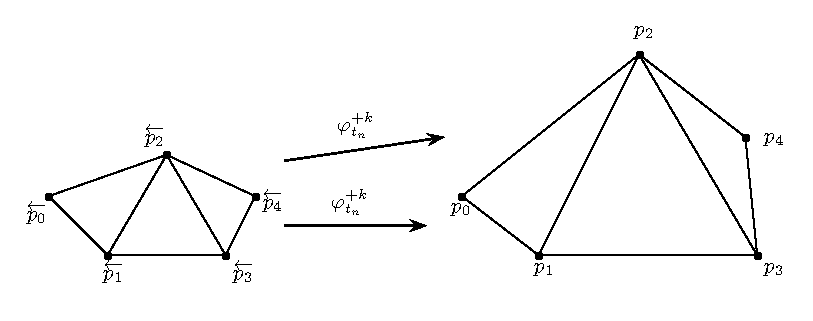
\includegraphics[width=0.45\linewidth]{pst/linearMARS1}
	}
	\hfill
	\subfigure[通过增加示踪点来使得三角形的边长都小于上界$h_L$]{
		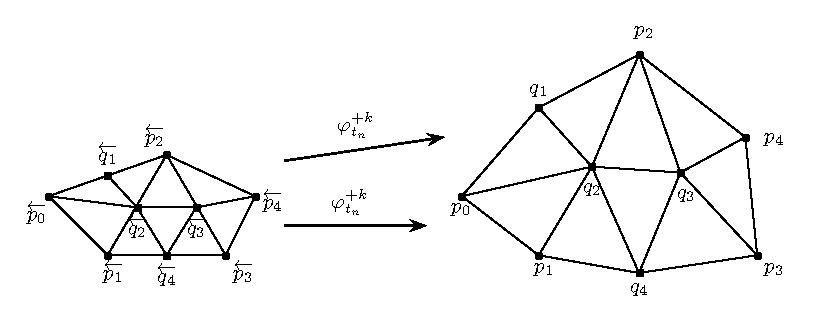
\includegraphics[width=0.45\linewidth]{pst/linearMARS2}
	}
	
	\subfigure[删除面积小于$\frac{r_ah_L^2}{2}$且超过两条边小于$r_{\mathsf{tiny}}h_L$的三角形]{
		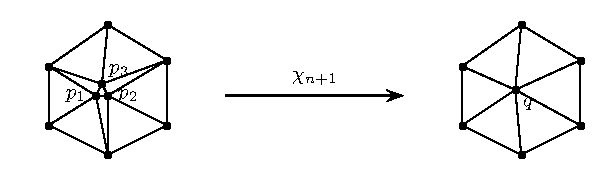
\includegraphics[width=0.45\linewidth]{pst/linearMARS3}
	}
	\hfill
	\subfigure[删除面积小于$\frac{r_ah_L^2}{2}$且只有一条边小于$r_{\mathsf{tiny}}h_L$的三角形]{
		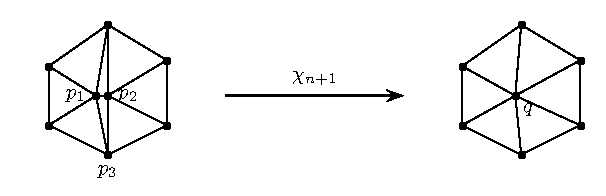
\includegraphics[width=0.45\linewidth]{pst/linearMARS4}
	}
	
	\subfigure[通过换边法优化三角形网格]{
		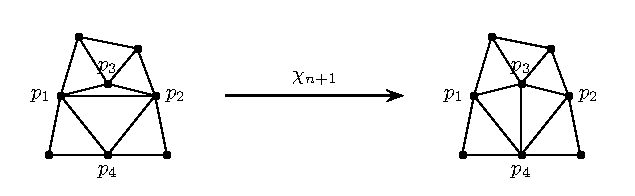
\includegraphics[width=0.45\linewidth]{pst/linearMARS5}
	}
	\hfill
	\subfigure[删除面积小于$\frac{r_ah_L^2}{2}$且三边均标准的三角形]{
		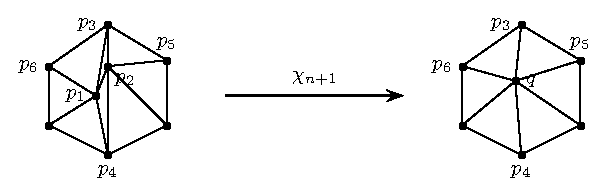
\includegraphics[width=0.45\linewidth]{pst/linearMARS6}
	}
	\caption[linear MARS方法的前三个步骤演示]{linear MARS方法的前三个步骤:
		在子图(a)中,
		界面 $\partial{\cal M}^n$上的示踪点被流映射$\varphi_{t_n}^{+k}$离散地映射到了像上.
		在子图(b)中,
		当 三角剖分中存在大于 $h_L$的边长的时候,
		通过添加示踪点来使得三角剖分的边长小于边长上界$h_L$.
		在子图 (c)中, 
		$\triangle_{p_1 p_2 p_3}$的面积小于  $\frac{r_ah_L^2}{2}$,
		且三边均小于$r_{\mathsf{tiny}}h_L.$ 
		将三角形 $\triangle_{p_1 p_2 p_3}$ 和另外三个与它共享一条边的三角形从三角剖分信息中删除,
		将顶点$p_1,p_2,p_3$用其重心来替换.
		在子图 (d)中,
		$\triangle_{p_1 p_2 p_3}$的面积小于$\frac{r_ah_L^2}{2}$, 
		其中$\overline{p_1 p_2}$小于边长下界,
		将$\overline{p_1 p_2}$ 缩成一个点,
		用其中点来替换点$p_1$, $p_2$ ,
		并把$\overline{p_1 p_2}$所在的两个三角形从三角剖分信息中删除.
		在子图 (e)中,
		三角形 $\triangle_{p_1 p_2 p_3}$的面积小于$\frac{r_ah_L^2}{2}$,
		通过换边法优化三角网格.
		在子图(f)中,
		换边法无法优化网格,
		则将三角形最小边用其中点替换.
	}
\end{figure}

\begin{defn}
	\label{defn:linMARS}
	在三维linear MARS方法中,
	用户需给出初始时刻流相边界的三角剖分信息作为其近似,
	并指定三角剖分中三角形边长界限$[r_\mathsf{tiny}h_L,h_L]$和三角形面积的下界$r_a$.
	三维linear MARS方法在每一个时间步$[t_n,t_n+k]$内,
	输入$\partial\mathcal{M}(t_n)$的三角剖分信息,
	通过以下步骤得到流相边界在$t_n+k$时刻的三角剖分信息作为对$\partial \mathcal{M}(t_{n+1})$的近似.

	\begin{enumerate}[{(linMARS}-1)]
		\setlength{\itemsep}{0pt}
		\setlength{\parsep}{0pt}
		\setlength{\parskip}{0pt}
		\item 对$\partial\mathcal{M}(t_n)$上的示踪点由流速场$\mathbf{u}$求解常微分方程
	           	     $\frac{\text{d}\mathbf{x}}{\text{d}t}=\mathbf{u}$
		             得到这些示踪点在$t_n+k$时刻的位置,记为$\{p_j\}$.
		\item 检查每一个三角形,若$\triangle_{p_i p_j p_k}$存在一条或一条以上的边大于上界$h_L$, 
		\begin{enumerate}[(a)]
			\item 在$\partial\mathcal{M}^n$上定位$\triangle_{p_i p_j p_k}$的顶点原像$\overleftarrow{p_i},
			             \overleftarrow{p_j}, \overleftarrow{p_k}$, 将大于上界$h_L$的边用其中点平分,并将这些中点标记为新的示踪点;
			\item 添加新边,用$\overleftarrow{p_i}, \overleftarrow{p_j}, \overleftarrow{p_k}$
			             和新的示踪点构建一个新的局部三角剖分;
			\item 用新的局部三角剖分来替代$\triangle_{p_i p_j p_k}$;
			\item 对于这些新的示踪点由流速场$\mathbf{u}$求解常微分方程
			            $\frac{\text{d}\mathbf{x}}{\text{d}t}=\mathbf{u}$得到这些新的示踪点
			            在$t_n+k$时刻的位置
			            并加入到顶点序列$\{p_j\}$中.
		\end{enumerate}
		重复以上步骤直到所有边长都不大于上界$h_L$.
		\item 检查每个三角形,若$\triangle_{p_i p_j p_k}$的面积小于$\frac{r_a \cdot h_L^2}{2}$
		             且满足删除条件(删除条件见下文分析),
		\begin{enumerate}
			\item 若三角形$\triangle_{p_i p_j p_k}$中有两条或以上的边小于$r_{\mathsf{tiny}}h_L$,
			             将该三角形缩成一个点;
			\item 若三角形$\triangle_{p_i p_j p_k}$仅有一边小于$r_{\mathsf{tiny}}h_L$,
			             将该边缩成一个点;
			\item 若三角形$\triangle_{p_i p_j p_k}$三条边都符合标准,用换边法优化网格,
			             若无法优化则将三角形的最小边缩成一个点.
		\end{enumerate}
	\item 得到一个新的三角剖分信息来近似$t_{n+1}$时刻的流相边界.
	\end{enumerate}
\end{defn}
在linear MARS中,显然(linMARS-3)中的三种处理方式
涵盖了所有面积小于$\frac{r_ah_L^2}{2}$且满足删除条件的三角形.


在定义\ref{defn:linMARS}中,
对于三角形的删除,我们还设置了可删除的限制条件.
如图3.2(a),
$p_0$是由$\triangle_{p_0 p_2 p_1}, \triangle_{p_0 p_3 p_2 }, \triangle_{p_0 p_1 p_3}$的交点,
$\triangle_{p_1 p_2 p_4}$与$\triangle_{p_0 p_2 p_1}$相交于$\overline{p_1 p_2}$,
当$\overline{p_1 p_2}$小于下界时,
若将其用中点$q$代替,
$\triangle_{p_0 p_1 p_3}$与$\triangle_{p_0 p_2 p_3}$的交是$\triangle_{p_0 q p_3}$,
网格不再是单纯复形,此时我们拒绝删除操作.
另外,当流向的局部变得极细的时候,为了保持其流相特征,
其附近的三角形可能很小,
如图3.2(b),
当$\overline{p_1p_2}$小于边长下界时,
若将其缩成一个点,三棱柱截断,流相的拓扑结构的改变.
由此可见,设置删除操作的限制是十分必要的.

\begin{figure}[htb]
	\label{fig:noDelete}
	\centering
	\subfigure[尖点附近的网格信息示例]{
		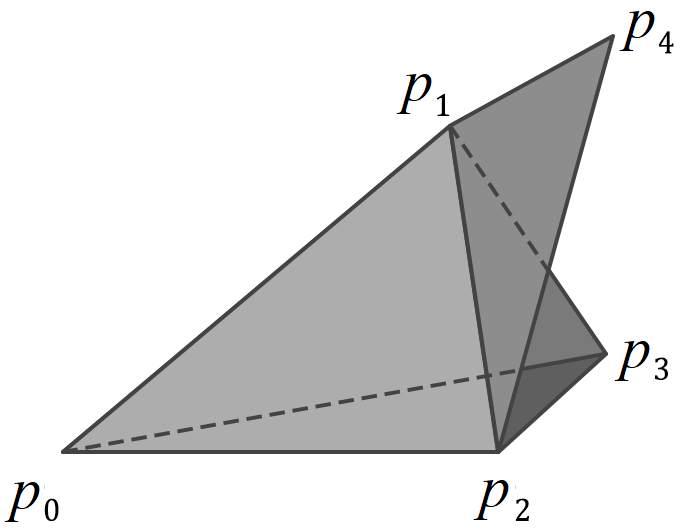
\includegraphics[width=0.4\linewidth]{images/111}
	}
	\hfill
	\subfigure[流相极细处的网格信息示例]{
		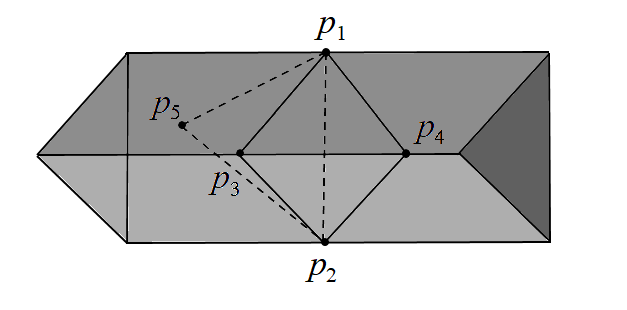
\includegraphics[width=0.4\linewidth]{images/333}
	}
	\caption{不满足删除条件的网格示例}
\end{figure}

假设$T$是所定位的要进行删除操作的三角形,
$T$是流相界面三角剖分的子复形,
对其进行删除操作所影响的区域很显然是在$\mathrm{star}(T)$范围内的,
因此在删除操作前,我们需要对$\mathrm{star}(T)$进行分析.
设集合$A=\{\mathbf{a}_1,\cdots,\mathbf{a}_i\}$是star$M$中所有三角形法向的集合,
定义$\mathrm{star}(T)$的平面最大夹角,
\begin{equation}
\label{defn:maxTheta}
\theta_T=\arccos(\min_{\textbf{a}_j\in A}|\mathbf{a}_T\cdot\mathbf{a}_j |).
\end{equation}
$\mathbf{a}_T$是三角形$T$的单位法向,
$\theta_T$直观地反应了$\mathrm{star}(T)$局部平面的平整程度,
当$\mathrm{star}(T)$趋于平整的时候,我们允许进行删除操作,
用户也可以自行指定$\cos\theta_T$的下界来限制删除操作的进行.
\begin{prop}
	linear MARS方法中流相界面的三角剖分在每一个时间步都是一个2-复形.
\end{prop}

\begin{proof}
(linMARS-2)中的(b)操作,保证了局部三角剖分是一个2-复形,
而(a)操作保证对每个局部三角剖分之间的公共边的处理一致,
因此(linMARS-2)保持了界面三角剖分是一个2-复形.
(linMARS-3)中的删除操作影响仅在$\mathrm{star}(T)$范围内,
分别考虑$\mathrm{star}(T)$内的2-单形和1-单形.
以图\ref{fig:linMARS}(d)的操作为例,
2-单形$\triangle_{p_1 p_2 p_3}$有三个1维面
$\overline{p_1 p_2}, \overline{p_1 p_3}, \overline{p_2 p_3}$.
首先考虑与$\triangle_{p_1 p_2 p_3}$的交集分别是1维面
$\overline{p_1 p_2}, \overline{p_1 p_3}, \overline{p_2 p_3}$的三个2-单形,
记作$\triangle_{p_1 p_2 p_4}, \triangle_{p_2 p_3 p_5}, \triangle_{p_1 p_3 p_6}$.
其中,2-单形$\triangle_{p_1 p_2 p_4}$塌缩成了1-单形.
又因$\triangle_{p_1 p_2 p_3}$塌缩成了一个1-单形$\overline{p_3 q}$,
$\triangle_{p_2 p_3 p_5}$的1维面$\overline{p_2 p_3}$
及$\triangle_{p_1 p_3 p_6}$的1维面$\overline{p_1 p_3}$均被$\overline{p_3 q}$替换,
因此$\overline{p_3 q}$是$\triangle_{p_1 p_3 p_6}$和$\triangle_{p_2 p_3 p_5}$的交.
当且仅当$\triangle_{p_2 p_3 p_5}$与$\triangle_{p_1 p_3 p_6}$的交
不包含除$\overline{p_3 q}$以外的1维面时,
网格保持是一个2-复形,而上述删除限制保证了这一条件.


对于$\mathrm{star}(T)$范围内的1-单形,
三个1-单形$\overline{p_1 p_2}, \overline{p_1 p_3}, \overline{p_2 p_3}$
塌缩成了一个1-单形$\overline{p_3 q}$,
$\triangle_{p_1 p_2 p_4}$与$\triangle_{p_1 p_2 p_3}$的交是$\overline{p_1 p_2}$,
又$\overline{p_1 p_2}$塌缩成了0-单形,
$\overline{p_4 q}$与$\overline{p_3 q}$相交于点$q$.
 而其他任意一个1-单形与$\overline{p_3 q}$的交集要么是空集,
 要么是单个0维面.
 假设存在一个1-单形$\overline{p_i p_j}$,
 其与$\overline{p_3 q}$的交集包含了两个或以上的点,
 则$\overline{p_i p_j}$至少与$\overline{p_1 p_2}, \overline{p_1 p_3}, \overline{p_2 p_3}$
 中的某一个1-单形的交集包含了两个或者以上的点,
 这与初始网格是一个单纯复形相矛盾,
 因此$\mathrm{star}(T)$范围内的任意两个1-单形都满足它们的交不是空集就是单个0维面.

综上,再由定义\ref{defn:simplex}可得
linear MARS中流相界面的三角剖分在每一个时间步都是一个2-复形.
\end{proof}

\section{linear MARS误差分析}
\begin{prop}
	\label{prop:error}
	(linear MARS方法的收敛性)三维空间上的linear MARS
	   在1-范数\eqref{defn:error}下是$2\alpha$精度的,
	    若其满足以下条件:
	\begin{enumerate}[(a)]
		\item 离散流映射$\mathring{ \phi}$在时间积分上至少是$2\alpha$阶精度的;
		\item 时间步长满足$k=O(h)$;
		\item $h_L=r_{\alpha} h^{\alpha}$满足$r_{\alpha}=O(1)$且$\alpha\geq 1$.
	\end{enumerate}
\end{prop}
\begin{proof}	
	根据\eqref{defn:accuracy}可得,
	linMARS的整体误差是多个单一误差的线性累加,
	因此我们只需对每个算子分别进行误差估计.
	通过(linMARS-2)和假设(b)和(c),在任意时间步,
	若界面上的两个相邻的顶点之间的最大距离为$h_{\mathrm{max}}=O(h^{\alpha})=O(k^{\alpha})$.
	根据误差定义\eqref{eq:geomError}得通过添加三角剖分中边的中点来作为新的示踪点不会增加误差,
	因此$E^{\textsf{AUG}}=0$.
	接下来证明任意时间步两个相邻点之间的最大距离$h_{\mathrm{max}}=O(h^{\alpha})$
	以及调整算子$\chi$带来的误差$E^{\textsf{ADJ}}=O(k^{2\alpha})$即可.
	
	
	由(linMARS-2)保证了当时相邻两个示踪点之间的距离最大为$h_L$. 
	(linMARS-3)中的删除操作会造成三角形顶点的偏移,
	从而造成相邻示踪点之间的距离扩大.
	但显然删除操作所造成的影响范围仅在删除三角形的星形范围内.
	当三角形面积小于$\frac{r_ah_L^2}{2}$时进行删除操作,
	所以在\ref{defn:linMARS}(f)中缩成点的边的长度有,
	\begin{equation*}
	l\leq\sqrt{\frac{h_L^2}{4}+(r_ah_L)^2}\leq(\frac{1}{2}+r_a)h_L.
	\end{equation*}
因此顶点的偏移距离最多为$\frac{1}{2}(\frac{1}{2}+r_a)h_L<h_L$,可得任意时间步内,
两个相邻示踪点之间的最大距离不超过$2h_L$,即$h_{\mathrm{max}}=O(h^{\alpha})$.
下证调整算子$\chi$带来的误差$E^{\textsf{ADJ}}=O(k^{2\alpha})$.

	 \begin{figure}[htbp]
		\label{fig:noDelete}
		\centering
			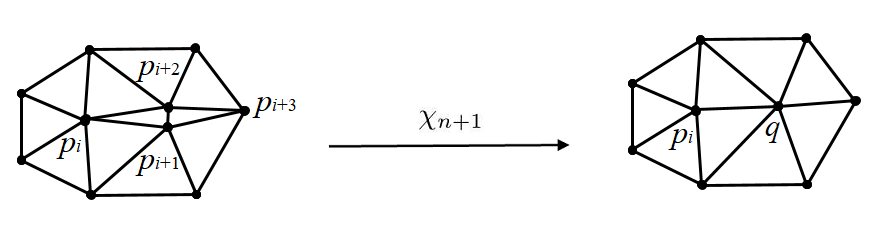
\includegraphics[width=0.7\linewidth]{images/error}
		\caption{调整算子误差分析图}
	\end{figure}
	
	如图3.3所示,记$\triangle_{p_i p_{i+1} p_{i+2}}$的星形为$\mathrm{star}(T)$,
	记调整之后的$\overline{p_i q}$的星形为$\mathrm{star}(E)$.
	调整算子在对于$\triangle_{p_i p_{i+1} p_{i+2}}$进行删除时,
	仅移动了$\triangle_{p_i p_{i+1} p_{i+2}}$上的两个顶点,
	而$\mathrm{star}(T)$边界上的顶点以及边并没有进行任何调整,
	因而$\mathrm{star}(T)$和$\mathrm{star}(E)$形成了一个闭合曲面,
	由\eqref{defn:error}可知调整算子所带来的误差是该闭合曲面所包围的体积.
	又由隐函数定理可得,一定存在一个投影平面,
	使得$\mathrm{star}(T)$和$\mathrm{star}(E)$均可以作为该投影平面上的连续二次函数,
	分别记为$F_1$和$F_2$,且$F_1$和$F_2$有相同的投影区域$D$.
	$\mathrm{star}(T)$和$\mathrm{star}(E)$形成的闭合曲面所包围的体积是,
	\begin{equation*}
	\int\int_{D}|F_1-F_2|\mathrm{d}\sigma.
	\end{equation*}
	由积分中值定理可得在$D$内,至少存在一点$(\varepsilon,\mu)$,使得
	\begin{eqnarray}
	\int\int_{D}|F_1-F_2|\mathrm{d}\sigma=|F_1(\varepsilon,\mu)-F_2(\varepsilon,\mu)|\cdot\sigma_0.
	\end{eqnarray}
	其中$\sigma_0$是该投影区域$D$的面积,是$O(h_L^2)$,
	因此该闭合曲面所包围的体积最大应是$O(h_L^4)$.
	由于在界面上的示踪点的数量为$O(\frac{1}{h_L^2})$,
	因而在每一个时间步执行次操作的次数最多是$O(\frac{1}{h_L^2})$,
	故调整算子$\chi$对与静态半代数集$\mathcal{P}$造成的误差是$O(h_L^2)$.
	当$\mathcal{P}$上存在$C_1$不连续点时,
	上述闭合曲面所包围的体积可能达到$O(h_L^3)$,
	但Sard定理指出$C_1$不连续的点至多只有常数个,
	因此上述对调整算子所带来的误差分析依然成立.
	
	
	综上所述,调整算子$\chi$对静态半代数集$\mathcal{P}$所造成的误差是$O(h_L^2)$. 
	由\eqref{lem:ADJerror}可得每个时间步都有$\|\varepsilon_n^{\textsf{ADJ}}\|=O(kh_L^2)$.
	因此,存在一个$c_k=O(1)$使得
	\begin{equation}
	E^{\textsf{ADJ}}\leq c_k\sum_{j-1}^n\|\varepsilon_j^{\textsf{ADJ}}\|=O(h^2).
	\end{equation}
	最后根据推论\eqref{cor:errorbound}命题得证.
\end{proof}
  \chapter{数值实验}
在本章中,我们进行了几个经典的测试并展示了测试结果.
在时间的积分上,我们采用的是经典的四阶龙格库塔方法.
对于测试的输入,即球面的三角剖分,我们通过以下方式得到.

\begin{figure}[htb]
	\label{fig:getTRI}
	\centering
	\subfigure[初始三角网格]{
		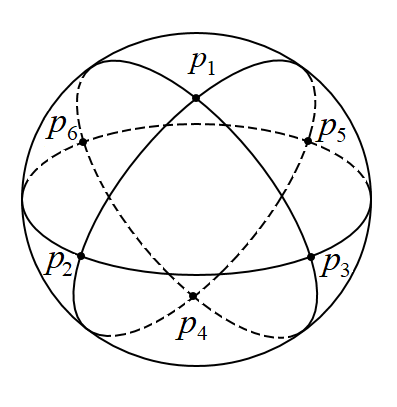
\includegraphics[width=0.4\linewidth]{images/ball}
	}
	\hfill
	\subfigure[对于初始三角网格的细化]{
		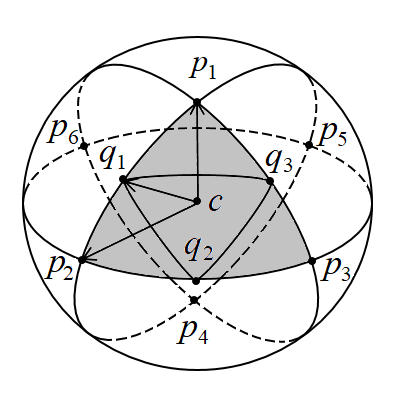
\includegraphics[width=0.4\linewidth]{images/ball3}
	}
	\caption{初始网格生成示意图}
\end{figure}

以球心是原点的单位球为例,在初始时刻给出所要剖分的球面的以下信息:
\begin{enumerate}
	\setlength{\itemsep}{0pt}
	\setlength{\parsep}{0pt}
	\setlength{\parskip}{0pt}
	\item 球心$c=(0,0,0)$,
	\item 半径$r=1$,
	\item 三角剖分信息(定义\ref{defn:triangulation}).
\end{enumerate}
三角剖分信息的给定不是唯一的,文中最初给定的三角剖分信息如下,见图4.1(a)
\begin{enumerate}
	\setlength{\itemsep}{0pt}
	\setlength{\parsep}{0pt}
	\setlength{\parskip}{0pt}
	\item 顶点个数$n_v=6$,三角形个数$n_t=8$;
	\item $6\times 3$的矩阵Pts,第$i$行表示了第$i$个顶点的坐标;
	\item $8\times 3$的矩阵,第$i$行的三个元素表示了第$i$个三角形的三个顶点在矩阵Pts中的指标.
\end{enumerate}
另外我们要求每个三角形的法向与其三个顶点满足右手法则,
并且所有三角形的法向朝球外部,这样做不仅利于计算多面体体积,
也为今后的殷集的布尔代数运算及样条曲面插值做铺垫.


在给出了初始的三角剖分之后,我们对其进行细化,
由于文中给出的初始三角剖分的每一个三角形都是正三角,
因此对于每个三角形我们都进行一致的细化操作.
以$p_1, p_2, p_3$所在的面为例,见图4.1(b).
已知球的球心为$c$,半径为$r$,则有

\begin{equation}
\left\{
\begin{array}{r}
\vec{cq_1}=r\cdot\frac{(\vec{cp_1}+\vec{cp_2})}{\|\vec{cp_1}+\vec{cp_2}\|},\\[0.2cm]
\vec{cq_2}=r\cdot\frac{(\vec{cp_2}+\vec{cp_3})}{\|\vec{cp_2}+\vec{cp_3}\|},\\[0.2cm]
\vec{cq_3}=r\cdot\frac{(\vec{cp_1}+\vec{cp_3})}{\|\vec{cp_1}+\vec{cp_3}\|}.\\[0.2cm]
\end{array}\right.
\end{equation}
$q_1, q_2, a_3$将$p_1, p_2, p_3$所在的三角曲面分割成四个三角曲面来达到初始网格的细化,
我们要求细化之后的网格依然满足右手法则,法向朝球外部.
通过对网格的多次细化来得到合适的球的三角剖分信息,
例如对初始三角剖分进行三次细化和四次细化得到了图4.2.

\begin{figure}[htb]
	\label{fig:refine}
	\centering
	\subfigure[初始网格进行三次细化之后的网格]{
		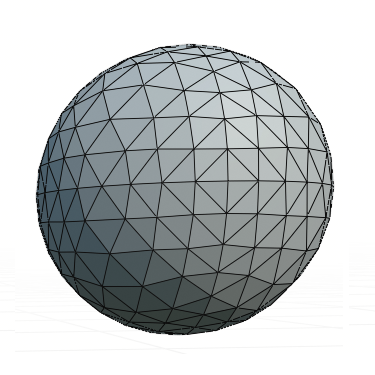
\includegraphics[width=0.4\linewidth]{images/3refine}
	}
	\hfill
	\subfigure[初始网格进行四次细化之后的网格]{
		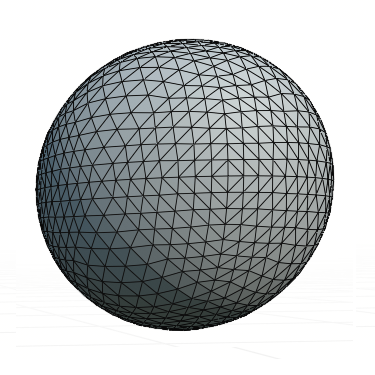
\includegraphics[width=0.4\linewidth]{images/4refine}
	}
	\caption{细化后的网格示意图}
\end{figure}


另外,由于直接求解1-范数\eqref{defn:error}较为困难,
在数值实验中,我们定义以下无穷范数和体积范数来作为准则,
\begin{equation}
E_{\infty}(T)=\max| r_i-r|.
\end{equation}
其中$r_i=\|p_i-C\|$,$p_i$是结束时刻所得流相界面的三角剖分上的顶点,
$C$是测试球的球心,$r$是测试球的半径.
\begin{equation}
E_{\mathrm{vol}}(T)=|V_{\mathrm{origin}}-V_{\mathrm{result}}|
\end{equation}
其中$V_{\mathrm{origin}}$是初始时刻用来近似流体的多面体体积,
$V_{\mathrm{result}}$是结束时刻所得的近似流体的多面体体积.



\section{二维剪切流场测试}
剪切流场中,$xy$方向上的流速由以下流函数给出,
\begin{equation*}
\psi (x,y)=-\frac{1}{\pi}\sin^2(\pi x)\sin^2(\pi y)\cos(\frac{\pi t}{T}),
\end{equation*}
而在$z$方向的速度为$0$, linear MARS在$\frac{T}{2}$时刻,
$x$和$y$方向上的流速符号被余弦项$\cos(\frac{\pi  t}{T})$反转,
因此在一个周期之后精确值与初始值完全一致,
测试参数见图\ref{tab:vortexSetup}.
在周期$T=8$的测试前半个阶段,
流相被速度场不断的拉伸变形成一个螺旋卷曲的薄片,
薄片向涡流中心旋转而存在被撕裂的可能.
这个测试中,尽管流体在几何上的形变很大,
但因流函数是同胚映射,流相不发生拓扑变化,
linear MARS方法良好的保持了剪切流场中流相的拓扑结构,
如图\ref{fig:vortexT8}.

\begin{figure}[htbp]
	\begin{minipage}[b]{0.65\linewidth}
		\renewcommand{\arraystretch}{1.2}
		\centering
		    \begin{tabular}{c|c}
      \hline
      参数名称 & 参数值  \\
      \hline
      测试区域     & $\Omega=[0,1]\times[0,1]\times[-0.5,0.5]$ \\
      测试时段 & $t\in[0,T]$ \\
      形状参数  & $C=(0.5,0.75,0.0)$, $R=0.15$ \\
      速度周期     & $T = 8$  \\
      库朗数 & $\text{Cr}=1$               \\
      控制体网格大小
      & $h = \frac{1}{16}, \frac{1}{32}, \frac{1}{64},  \frac{1}{128}$  \\
      界面尺度
      & $h_L= O(h), O(h^{\frac{3}{2}}), O(h^2)$, $r_{\mathsf{tiny}}=0.01$
      \\
      \hline
      \multicolumn{2}{c}{}\\
    \end{tabular}

%%% Local Variables: 
%%% mode: latex
%%% TeX-master: "../cubicMARS"
%%% End: 

	\end{minipage}
	\hfill
	\begin{minipage}{0.3\linewidth}
		\centering
		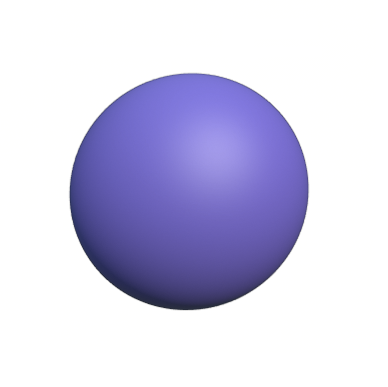
\includegraphics[width=1\linewidth]{images/3}
	\end{minipage}
	\caption{二维剪切流场测试参数}
	\label{tab:vortexSetup}
\end{figure}



\begin{figure}[htbp]
	\centering
	\subfigure[$t=0$]{
		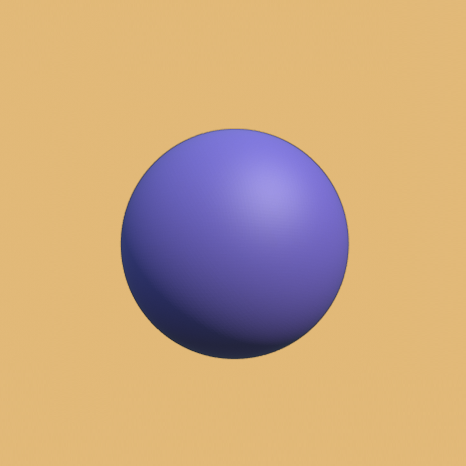
\includegraphics[width=0.305\linewidth]{images/v1}
	}
	\hfill
	\subfigure[$t=\frac{1}{8}T$]{
		
\includegraphics[width=0.305\linewidth]{images/v2}
	}
	\hfill
	\subfigure[$t=\frac{1}{4}T$]{
		
\includegraphics[width=0.305\linewidth]{images/v3}
	}
	
	\subfigure[$t=\frac{1}{2}T$]{
		
\includegraphics[width=0.30\linewidth]{images/v4}
	}
	\hfill
	\subfigure[$t=\frac{3}{4}T$]{
		
\includegraphics[width=0.305\linewidth]{images/v5}
	}
	\hfill
	\subfigure[$t=T$]{
		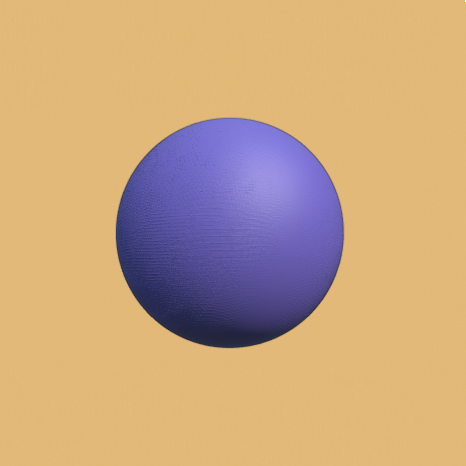
\includegraphics[width=0.305\linewidth]{images/v6}
	}
	\caption[二维剪切流场测试结果]{$T=8,r_{\mathsf{tiny}}=0.01,h_L=1/128$时,
		二维剪切流场的测试结果图.$(n_v,n_t)$在$T=0, \frac{T}{2}, T$时刻的值分别是$(16386,32768)$,$(272023,544042)$和$(166696,333388)$,
		$t=T$时刻的误差$E_{\infty}=4.11e-04,E_{\mathrm{vol}}=1.34e-06$.}
	\label{fig:vortexT8}
\end{figure}

%\begin{table}[htbp]
%	\label{tab1}
%	\centering
%	\caption[二维剪切流场的误差测试结果]{当$r_{\mathrm{tiny}}=0.01$时,二维剪切流场测试的误差结果}
%	\begin{tabular}{c|ccccccc}
%		\hline \hline
%		%    \multicolumn{2}{c|}{\rule[-3mm]{0mm}{8mm} Methods }
%		%Methods
%		&$h=\frac{1}{16}$ & rate & $h=\frac{1}{32}$ 
%		& rate & $h=\frac{1}{64}$ & rate &  $h=\frac{1}{128}$
%		\\ \hline 
%		& \multicolumn{6}{c}{$T=2$ }
%		\\ \hline 
%		$h_L=0.5h,E_{\infty}$ & 1.15e-03 & 1.91 & 3.05e-04 & 1.88&8.30e-05 & 2.05 & 2.00e-05
%		\\
%		$h_L=0.5h,E_{\mathrm{vol}}$  & 4.31e-06 & 1.92 & 1.14e-06 & 1.84 &3.18e-07 & 1.94 & 8.26e-08
%		\\ \hline 
%		$h_L=8h^{\frac{3}{2}},E_{\infty}$ & - & -  & 3.42e-03 & 2.77& 5.03e-04 & 3.13 & 5.73e-05
%		\\
%		$h_L=8h^{\frac{3}{2}},E_{\mathrm{vol}}$  & - & - & 2.70e-05 & 4.39 &1.29e-06& 2.46 & 2.34e-07
%		\\ \hline 
%		$h_L=64h^2,E_{\infty}$ & - & - & 2.78e-03 & 3.19 &3.05e-04 & 3.93 & 2.00e-05
%		\\
%		$h_L=64h^2,E_{vol}$  & - & - & 1.05e-05 & 3.02 &1.29e-06 & 3.97 & 8.26e-08
%		\\ \hline 
%		& \multicolumn{6}{c}{$T=4$ }
%		\\ \hline 
%		$h_L=0.5h,E_{\infty}$ & 1.74e-03 & 2.00 & 6.96e-04 & 2.00 &1.74e-04 & 2.00 & 4.36e-05
%		\\
%		$h_L=0.5h,E_{vol}$  & 1.18e-05 & 1.99 & 3.20e-06 & 2.07 &7.61e-07 & 2.00 & 1.90e-07
%		\\ \hline 
%		$h_L=8h^{\frac{3}{2}},E_{\infty}$ & - & - & 5.93e-03 & 3.09 &6.95e-04 & 2.90 & 9.30e-05
%		\\
%		$h_L=8h^{\frac{3}{2}},E_{\mathrm{vol}}$  & - & - & 4.51e-05 & 3.75 &00e-00 & 2.69 & 4.92e-07
%		\\ \hline 
%		$h_L=64h^2,E_{\infty}$ & - & - & 1.20e-02 & 4.11 &6.95e-04 & 3.99 & 4.36e-05
%		\\
%		$h_L=64h^2,E_{vol}$  & - & - & 5.78e-05 & 4.2 &3.14e-06 & 4.06 & 1.88e-07
%		\\ \hline 
%		& \multicolumn{6}{c}{$T=8$ }
%		\\ \hline 
%		$h_L=0.5h,E_{\infty}$ & 6.46e-03 & 2.00 & 1.62e-03 & 1.98 &4.11e-04 & 2.01 & 1.02e-04
%		\\
%		$h_L=0.5h,E_{vol}$   & 1.96e-05 & 2.15 & 4.43e-06 & 1.72 &1.34e-06 & 2.08 & 3.17e-07
%		\\ \hline 
%		$h_L=8h^{\frac{3}{2}},E_{\infty}$ & - & - & 1.41e-02 & 3.46 &1.28e-03 & 2.89 & 1.72e-04
%		\\
%		$h_L=8h^{\frac{3}{2}},E_{\mathrm{vol}}$ &- & - & 5.77e-05 & 3.64 &4.63e-06 & 2.14 & 1.05e-06
%		\\ \hline 
%		$h_L=64h^2,E_{\infty}$ & - & - & 2.66e-04 & 4.04 &1.62e-03 & 3.98 & 1.03e-04
%		\\
%		$h_L=64h^2,E_{vol}$  & - & - & 7.01e-05 & 3.92 &4.63e-06 & 3.87 & 3.17e-07
%		\\ \hline \hline
%	\end{tabular}
%\end{table}  

\begin{table}[htbp]
	\label{tab1}
	\centering
	\caption[二维剪切流场测试的误差结果]{当$r_{\mathsf{tiny}}=0.01$时,二维剪切流场测试的误差结果}
	\begin{tabular}{c|ccccccc}
		\hline \hline
		%    \multicolumn{2}{c|}{\rule[-3mm]{0mm}{8mm} Methods }
		%Methods
		&$h=\frac{1}{16}$ & rate & $h=\frac{1}{32}$ 
		& rate & $h=\frac{1}{64}$ & rate &  $h=\frac{1}{128}$
		\\ \hline 
		$h_L=0.5h,E_{\infty}$ & 6.46e-03 & 2.00 & 1.62e-03 & 1.98 &4.11e-04 & 2.01 & 1.02e-04
		\\
		$h_L=0.5h,E_{vol}$   & 1.96e-05 & 2.15 & 4.43e-06 & 1.72 &1.34e-06 & 2.08 & 3.17e-07
		\\ \hline 
		$h_L=8h^{\frac{3}{2}},E_{\infty}$ & - & - & 1.41e-02 & 3.46 &1.28e-03 & 2.89 & 1.72e-04
		\\
		$h_L=8h^{\frac{3}{2}},E_{\mathrm{vol}}$ &- & - & 5.77e-05 & 3.64 &4.63e-06 & 2.14 & 1.05e-06
		\\ \hline 
		$h_L=64h^2,E_{\infty}$ & - & - & 2.47e-04 & 3.93 &1.62e-03 & 3.99 & 1.02e-04
		\\
		$h_L=64h^2,E_{vol}$  & - & - & 7.01e-05 & 3.92 &4.63e-06 & 3.87 & 3.17e-07
		\\ \hline \hline
	\end{tabular}
\end{table}  

基于误差范数$E_{\infty}$和$E_{\mathrm{vol}}$,当$\alpha $分别取$1, \frac{3}{2}, 2$时,linear MARS方法基本上呈现了二、三、四阶精度,见表\ref{tab1}.
%在剪切流场的测试中,周期越长,流体的形变也就越大.从表$\ref{tab1}$中可得,当网格大小相同时,流相的形变越小,最终的误差$E_{\infty}$和$E_{\mathrm{vol}}$也越小.另外,基于误差范数$E_{\infty}$和$E_{\mathrm{vol}}$,当$\alpha $分别取$1, \frac{3}{2}, 2$时,linear MARS方法基本上呈现了二、三、四阶精度,见表\ref{tab1}.
\newpage

\section{二维变形流场测试}
变形流场测试被认为是界面追踪中最困难的问题之一.
其在$xy$方向上的流速由以下流函数得出,
\begin{equation*}
\label{eq:deformation}
\psi(x,y)=\frac{1}{n_{\mathrm{v}} \pi}\sin(n_{\mathrm{v}}(x+0.5))\cos(n_{\mathrm{v}}\pi(y+0.5))\cos(\frac{\pi t}{T}),
\end{equation*}
在$z$方向上的流速为$0$, $n_{\mathrm{v}}$表示在计算域中的涡流数,
流速符号在$\frac{T}{2}$时刻被余弦项$\cos(\frac{\pi  t}{T})$反转,
结束时刻其精确值与初始时刻一致,测试参数见图\ref{tab:deformation}.
在测试前半个周期中,流相的多个局部区域被流速场拉伸的很薄,
而linear MARS始终保持了流相的拓扑结构,如图\ref{fig:deformation}.
\begin{figure}[htbp]
	\begin{minipage}[b]{0.65\linewidth}
		\renewcommand{\arraystretch}{1.2}
		\centering
		    \begin{tabular}{c|c}
      \hline
      参数名称 & 参数值  \\
      \hline
      测试区域     & $\Omega=[0,1]\times[0,1]\times[-0.5,0.5]$ \\
      测试时段 & $t\in[0,T]$ \\
      形状参数  & $C=(0.5,0.5,0.0)$, $R=0.15$ \\
      速度参数    & $T = 2,n_{\mathrm{v}}=4$  \\
      库朗数 & $\text{Cr}=1$               \\
      控制体网格大小
      & $h = \frac{1}{16}, \frac{1}{32},\frac{1}{64},\frac{1}{128}$  \\
      界面尺度
      & $h_L= O(h), O(h^{\frac{3}{2}}), O(h^2)$, $r_{\mathsf{tiny}}=0.01$
      \\
      \hline
      \multicolumn{2}{c}{}\\
    \end{tabular}

%%% Local Variables: 
%%% mode: latex
%%% TeX-master: "../cubicMARS"
%%% End: 

	\end{minipage}
	\hfill
	\begin{minipage}{0.3\linewidth}
		\centering
		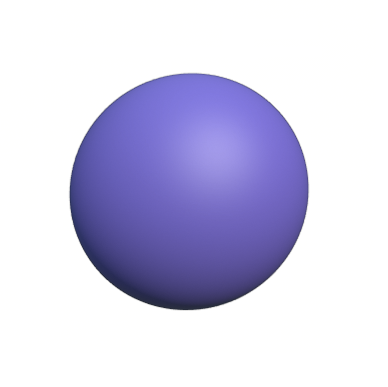
\includegraphics[width=1\linewidth]{images/3}
	\end{minipage}
	\caption{二维变形流场测试参数}
	\label{tab:deformation}
\end{figure}


\begin{figure}[htbp]
	\centering
	\subfigure[$t=0$]{
      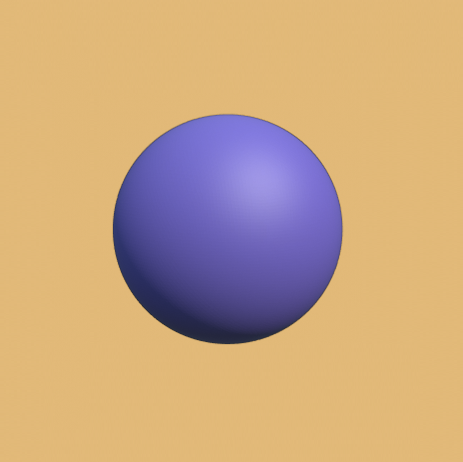
\includegraphics[width=0.315\linewidth]{images/d1}
	}
	\hfill
	\subfigure[$t=\frac{1}{8}T$]{
	  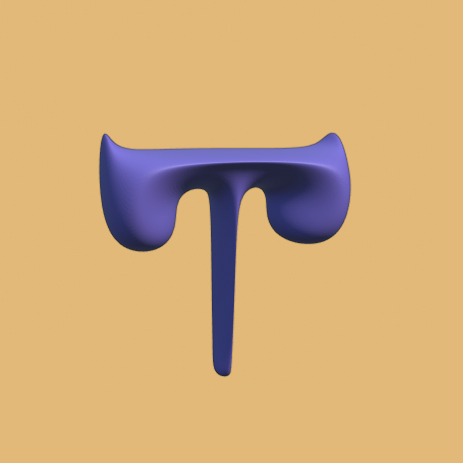
\includegraphics[width=0.315\linewidth]{images/d2}
	}
	\hfill
	\subfigure[$t=\frac{2}{8}T$]{
	  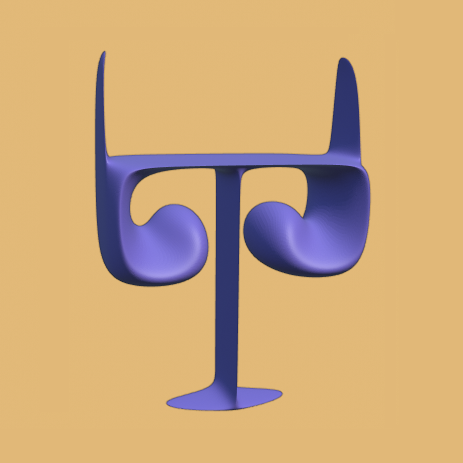
\includegraphics[width=0.315\linewidth]{images/d3}
	}
	
	\subfigure[$t=\frac{3}{8}T$]{
	  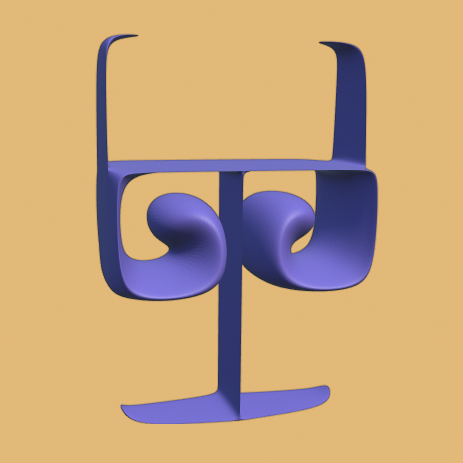
\includegraphics[width=0.315\linewidth]{images/d4}
	}
	\hfill
	\subfigure[$t=\frac{4}{8}T$]{
	  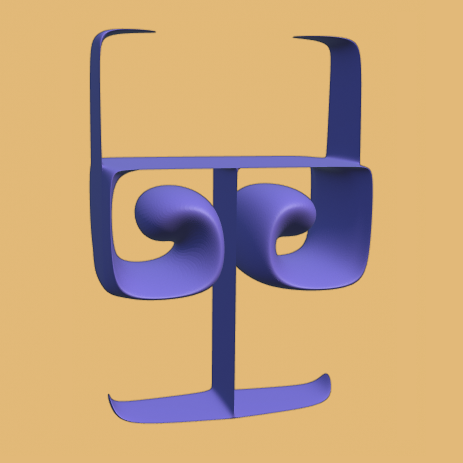
\includegraphics[width=0.315\linewidth]{images/d5}
	}
	\hfill
	\subfigure[$t=\frac{5}{8}T$]{
	  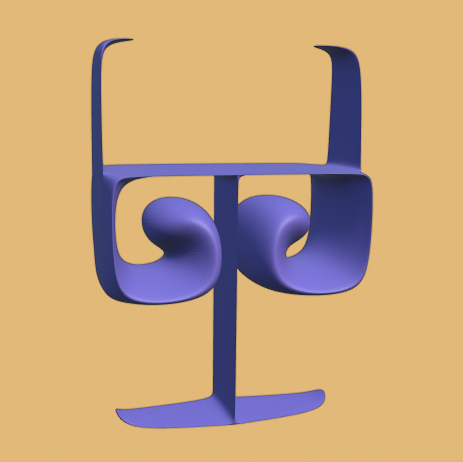
\includegraphics[width=0.315\linewidth]{images/d6}
	}
  	
  \subfigure[$t=\frac{6}{8}T$]{
  	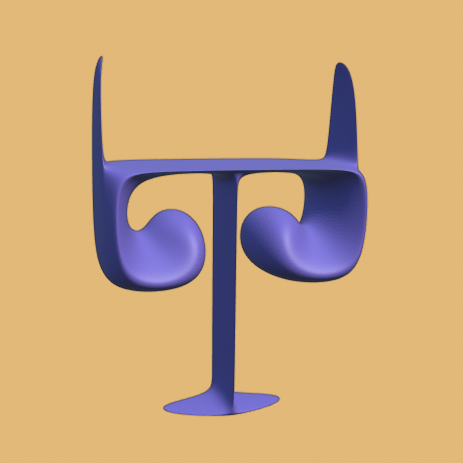
\includegraphics[width=0.315\linewidth ]{images/d7}
  }
  \hfill
  \subfigure[$t=\frac{7}{8}T$]{
   	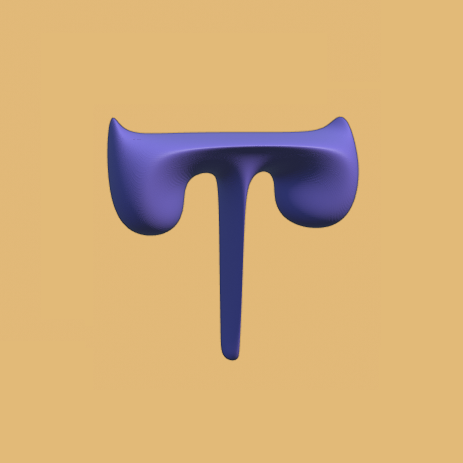
\includegraphics[width=0.315\linewidth ]{images/d8}
  }
  \hfill
  \subfigure[$t=T$]{
  	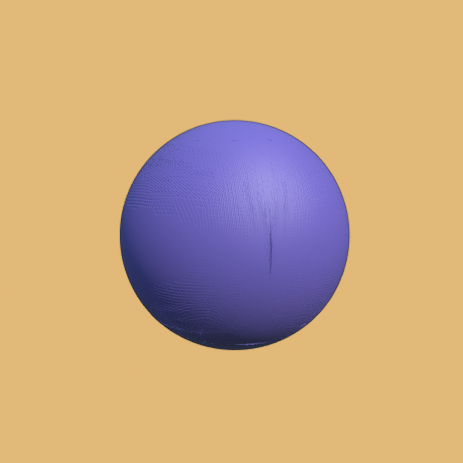
\includegraphics[width=0.315\linewidth ]{images/d9}
  }
	\caption[二维变形流场测试结果]{$T=2,n_{\mathrm{v}}=4,r_{\mathsf{tiny}}=0.01,h_L=1/128$时,
		二维变形流场的测试结果图.$(n_v,v_t)$在$T=0, \frac{T}{2}, T$时刻的值分别是$(16386,32768)$,$(444236,888468)$和$(116147,232290)$,
		$t=T$时刻的误差$E_{\infty}=5.81e-04,E_{\mathrm{vol}}=5.39e-07$.}
	\label{fig:deformation}
\end{figure}


\begin{table}[htb]
	\label{tab2}
	\centering
	\caption[二维变形流场测试的误差结果]{当$r_{\mathsf{tiny}}=0.01$时,二维变形流场测试的误差结果}
	\begin{tabular}{c|ccccccc}
		\hline \hline
		%    \multicolumn{2}{c|}{\rule[-3mm]{0mm}{8mm} Methods }
		linear MARS
		&$h=\frac{1}{16}$ & rate & $h=\frac{1}{32}$ 
		& rate & $h=\frac{1}{64}$ & rate &  $h=\frac{1}{128}$
		\\ \hline 
		& \multicolumn{6}{c}{$T=2,v_{\mathrm{v}}=4$ }
		\\ \hline 
		$h_L=h,E_{\infty}$ & 3.12e-02 & 1.93 & 8.16e-03 & 2.01 &2.03e-03 & 1.80& 5.81e-04
		\\
		$h_L=h,E_{\mathrm{vol}}$  & 2.42e-05 & 1.56 & 8.18e-06 & 1.63 &2.64e-06 & 2.29 & 5.39e-07
		\\ \hline 
		$h_L=8h^{\frac{3}{2}},E_{\infty}$ & - & - & 1.40e-02 & 2.79 & 2.03ee-03 & 2.57 & 3.43e-04
		\\
		$h_L=8h^{\frac{3}{2}},E_{\mathrm{vol}}$  & - & - & 8.93e-06 & 2.55 &1.53e-06 & 4.16 & 8.55e-08
		\\ \hline 
		$h_L=64h^2,E_{\infty}$ & - & - & 3.10e-02 &3.93 &2.03e-03 & 2.94 & 2.65e-04
		\\
		$h_L=64h^2,E_{\mathrm{vol}}$  & - & - & 2.69e-05 & 3.90 &1.80e-06 & 4.01 & 1.12e-07
		\\ \hline \hline
	\end{tabular}
\end{table}  

变形流场测试中,基于误差范数$E_{\infty}$和$E_{\mathrm{vol}}$,
当$\alpha$分别取$1,\frac{3}{2},2$时,linear MARS总体上呈现了二、三、四精度,
但也存在着个别测试没有达到理论精度.
这可能是由于流相在测试中的形变过大,造成了精度的降低,见表\ref{tab2}.


\section{三维剪切流场测试}
LeVeque\cite{leveque96}通过叠加$xy$平面上的形变与$xz$平面上的形变,
将二维的剪切流场扩展到了三维,提出了一个在三维空间中的不可压流场,
其三个方向的流速如下:
\begin{equation*}\label{bilevel}
\left\{\begin{array}{l}
v_x(x,y,z,t)=\cos(\frac{\pi  t}{T})2\sin^2(\pi x)\sin(2\pi y)\sin(2\pi z),\\[0.2cm]
v_y(x,y,z,t)=-\cos(\frac{\pi t}{T})\sin(2\pi x)\sin^2(\pi y)\sin(2 \pi z),\\[0.2cm]
v_z(x,y,z,t)=-\cos(\frac{\pi t}{T})\sin(2\pi x)\sin(2\pi y)\sin^2(\pi z).\\[0.2cm]
\end{array}\right.
\end{equation*}


流体的运动周期依赖于$\cos(\frac{\pi t}{T})$这一项.
同样的,流相在$\frac{T}{2}$时刻反转,
因此其在周期结束时刻恢复初始值,测试参数见图\ref{tab:de3}.
在测试的前半个周期,
球体被两个旋转的涡流夹带,
漩涡从两个相反方向作用于球体两侧,
并且挤压球体,
使球体变得很薄且形变后的流体两端变得十分伸展,
见图\ref{fig:3Dflow}.
LS方法对于处理这样的薄的界面追踪时,
最终结果可能改变流相的拓扑结构\cite{enright02:_hybrid_partic_level_set_method},
而linear MARS方法很好的保持了流相的拓扑信息.
\begin{figure}[htbp]
	\begin{minipage}[b]{0.65\linewidth}
		\renewcommand{\arraystretch}{1.2}
		\centering
		    \begin{tabular}{c|c}
      \hline
      参数名称 & 参数值  \\
      \hline
      测试区域     & $\Omega=[0,1]\times[0,1]\times[-0.5,0.5]$ \\
      测试时段 & $t\in[0,T]$ \\
      形状参数  & $C=(0.35,0.35,0.35)$, $R=0.15$ \\
      速度参数    & $T = 3$\\
      库朗数 & $\text{Cr}=1$               \\
      控制体网格大小
      & $h =  \frac{1}{16}, \frac{1}{32}, \frac{1}{64}, \frac{1}{128}$  \\
      界面尺度
      & $h_L= O(h), O(h^{\frac{3}{2}}),O(h^2)$, $r_{\mathrm{tiny}}=0.01,0.1$
      \\
      \hline
      \multicolumn{2}{c}{}\\
    \end{tabular}

%%% Local Variables: 
%%% mode: latex
%%% TeX-master: "../cubicMARS"
%%% End: 

	\end{minipage}
	\hfill
	\begin{minipage}{0.3\linewidth}
		\centering
		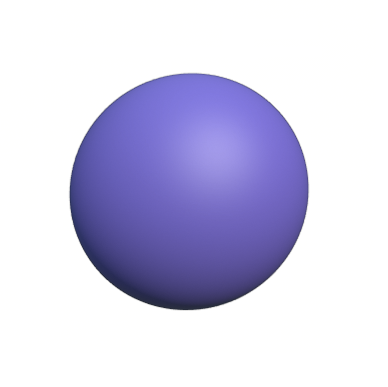
\includegraphics[width=1\linewidth]{images/3}
	\end{minipage}
	\caption{三维剪切流场测试参数}
	\label{tab:de3}
\end{figure}
%\begin{figure}
%	\label{fig:de3}
%	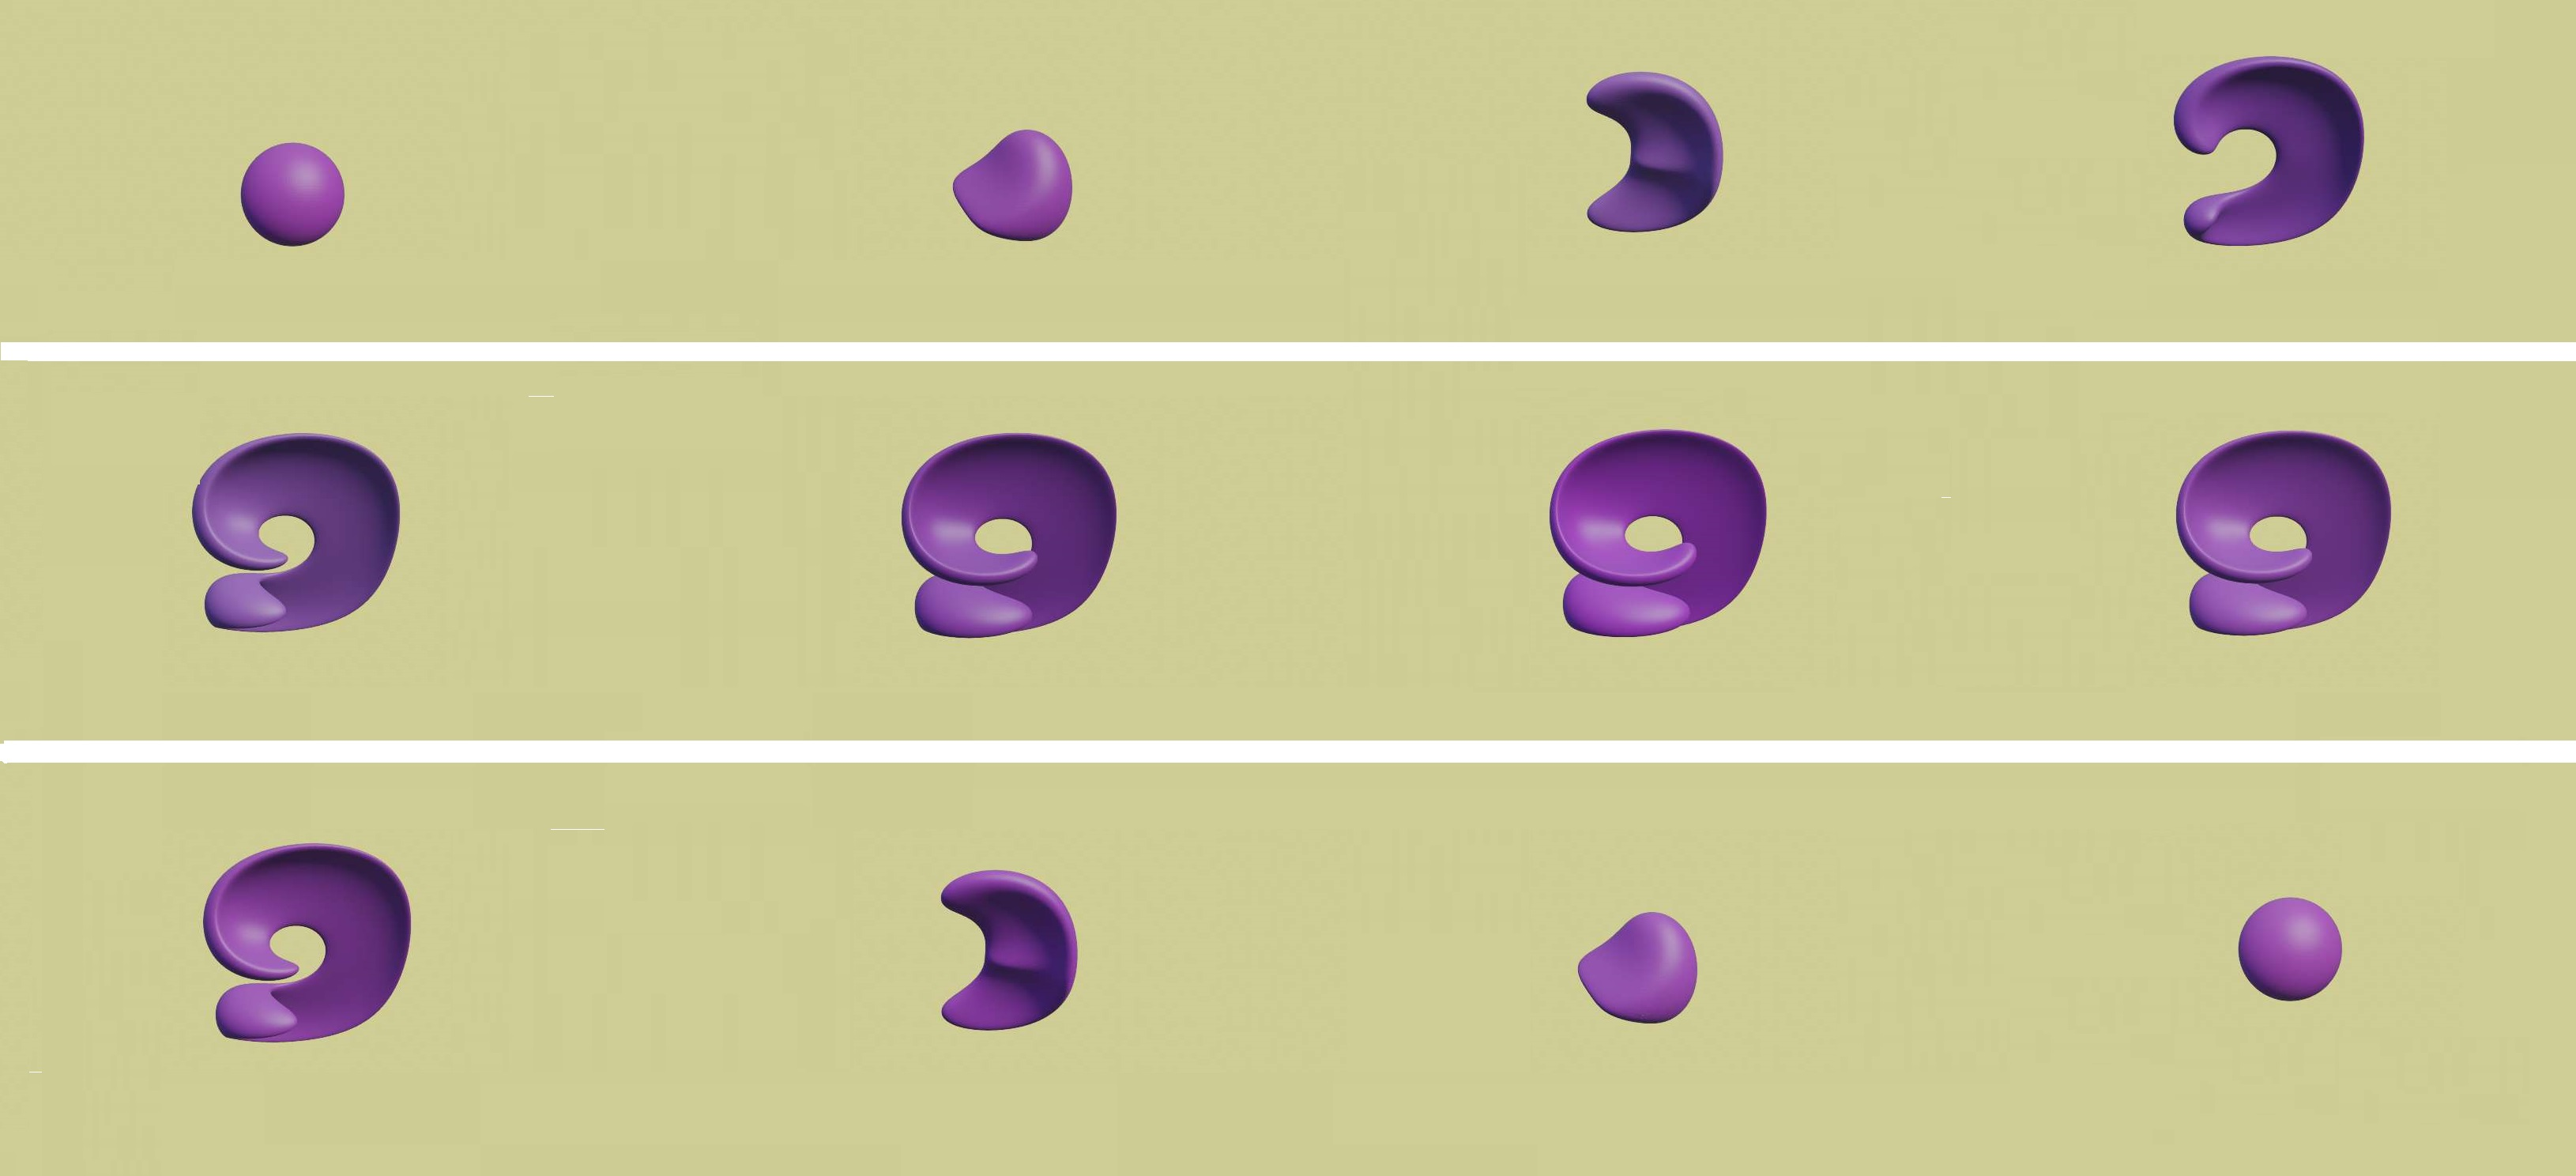
\includegraphics[width=\linewidth]{images/三维渲染图}
%	\caption[三维变形流场测试结果]{$h_L=1/128$时,三维变形流场测试中流相的形变过程图}
%\end{figure}

\begin{table}[htbp]
	\label{tab3}
	\centering
	\caption[$r_{\mathsf{tiny}}=0.01$时,三维剪切流场测试的误差结果]{当$r_{\mathsf{tiny}}=0.01$时,
		三维变形流场测试的误差结果}
	\begin{tabular}{c|ccccccc}
		\hline \hline
		%    \multicolumn{2}{c|}{\rule[-3mm]{0mm}{8mm} Methods }
		linear MARS
		&$h=\frac{1}{16}$ & rate & $h=\frac{1}{32}$ 
		& rate & $h=\frac{1}{64}$ & rate &  $h=\frac{1}{128}$
		\\ \hline 
		$h_L=0.5h,E_{\infty}$ & 6.03e-03 & 2.21 & 1.30e-03 & 2.10 &3.03e-04 & 1.95 & 7.85e-05
		\\
		$h_L=0.5h,E_{\mathrm{vol}}$  & 2.97e-05 & 2.65 & 4.73e-06 & 2.09 &1.12e-06 & 1.87 & 3.06e-07
		\\ \hline 
		$h_L=8h^{\frac{3}{2}},E_{\infty}$ & - & - & 1.00e-02 & 2.95 &1.29e-03 & 3.26 & 1.35e-04
		\\
		$h_L=8h^{\frac{3}{2}},E_{\mathrm{vol}}$  & - & - & 7.08e-05 & 3.72 &5.39e-06 & 3.25 & 5.67e-07
		\\ \hline 
		$h_L=64h^2,E_{\infty}$ & - & - & 2.62e-02 & 4.33 &1.30e-03 & 4.05 & 7.85e-05
		\\
		$h_L=64h^2,E_{\mathrm{vol}}$  & - & - & 9.27e-05 & 4.10 &5.39e-06 & 4.14 & 3.06e-07
		\\ \hline \hline
	\end{tabular}
\end{table}  

\begin{table}[htbp]
	\label{tab4}
	\centering
		\caption[$r_{\mathsf{tiny}}=0.1$时,三维剪切流场测试的误差结果]{当$r_{\mathsf{tiny}}=0.1$时,
			三维剪切流场测试的误差结果}
	\begin{tabular}{c|ccccccc}
		\hline \hline
		%    \multicolumn{2}{c|}{\rule[-3mm]{0mm}{8mm} Methods }
		linear MARS
		&$h=\frac{1}{16}$ & rate & $h=\frac{1}{32}$ 
		& rate & $h=\frac{1}{64}$ & rate &  $h=\frac{1}{128}$
		\\ \hline 
		$h_L=0.5h,E_{\infty}$ & 1.96e-02 & 2.19 & 4.30e-03 &1.53&1.49e-03& 1.33 & 5.93e-04
		\\
		$h_L=0.5h,E_{\mathrm{vol}}$  & 3.05e-04 & 1.90 & 8.17e-05 & 1.87 &2.23e-05 & 1.93 & 5.86e-06
		\\ \hline 
		$h_L=8h^{\frac{3}{2}},E_{\infty}$ & - & - & 3.69e-02 & 3.13 &4.21e-03 & 2.11 & 9.76e-04
		\\
		$h_L=8h^{\frac{3}{2}},E_{\mathrm{vol}}$  & - & - & 5.14e-04 & 2.59&8.53e-05 & 2.83 & 1.20e-05
		\\ \hline 
		$h_L=64h^2,E_{\infty}$ & - & - & 6.02e-02 & 3.84 &4.21e-03 & 2.83 & 5.93e-04
		\\
		$h_L=64h^2,E_{\mathrm{vol}}$  & - & - & 9.44e-04 & 3.44 &8.70e-05 & 3.88 & 5.89e-06
		\\ \hline \hline
	\end{tabular}
\end{table}  

三维变形流场测试中,基于误差范数$E_{\infty}$和$E_{\mathrm{vol}}$,
当$r_{\mathsf{tiny}}=0.01$,$\alpha$分别取值$1,\frac{3}{2},2$时,
linear MARS方法分别呈现出了二、三、四阶精度,见表\ref{tab3}.
当$r_{\mathsf{tiny}}=0.1$时,
测试的运行时间降低,而最终的误差有所加大,
同时精度也有所下降,见表\ref{tab4}.

\begin{figure}[htbp]
	\centering
	\subfigure[$t=0$]{
		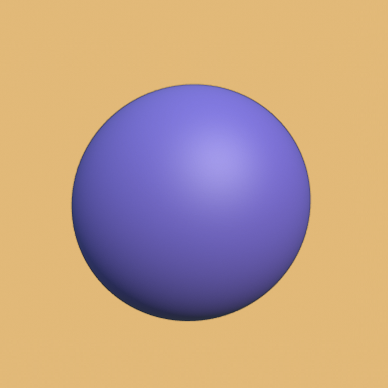
\includegraphics[width=0.3\linewidth]{images/3d-1}
	}
	\hfill
	\subfigure[$t=\frac{1}{8}T$]{
		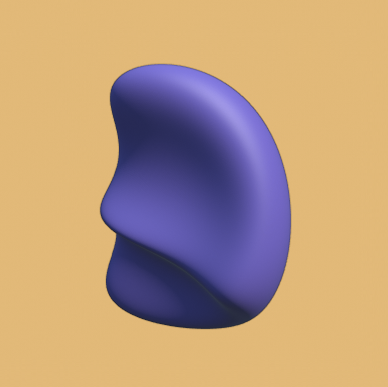
\includegraphics[width=0.3\linewidth]{images/3d-2}
	}
	\hfill
	\subfigure[$t=\frac{2}{8}T$]{
		
\includegraphics[width=0.3\linewidth]{images/3d-3}
	}
	
	\subfigure[$t=\frac{3}{8}T$]{
		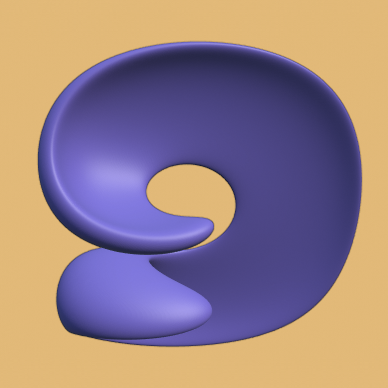
\includegraphics[width=0.3\linewidth]{images/3d-4}
	}
	\hfill
	\subfigure[$t=\frac{4}{8}T$]{
		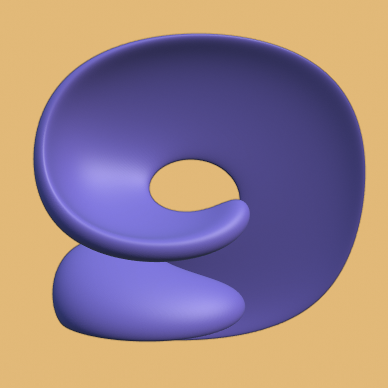
\includegraphics[width=0.3\linewidth]{images/3d-5}
	}
	\hfill
	\subfigure[$t=\frac{5}{8}$]{
		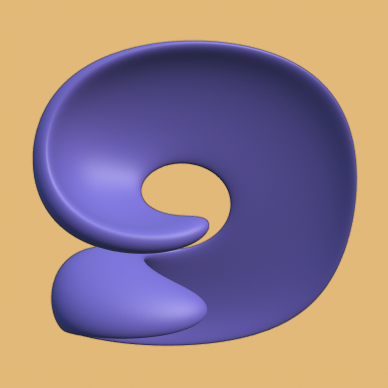
\includegraphics[width=0.3\linewidth]{images/3d-6}
	}
	
	\subfigure[$t=\frac{6}{8}T$]{
		
\includegraphics[width=0.3\linewidth ]{images/3d-7}
	}
	\hfill
	\subfigure[$t=\frac{7}{8}T$]{
		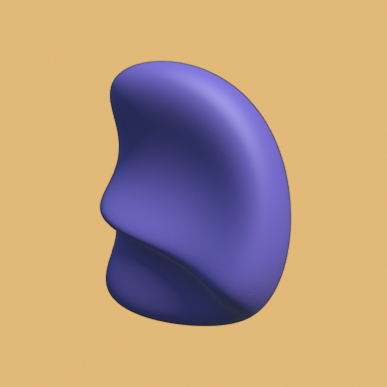
\includegraphics[width=0.3\linewidth ]{images/3d-8}
	}
	\hfill
	\subfigure[$t=T$]{
		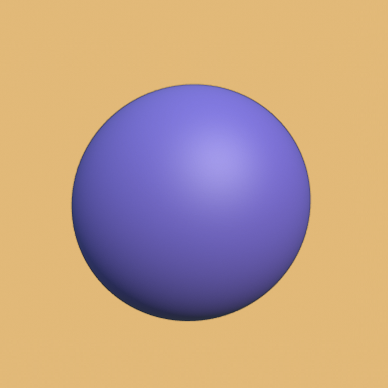
\includegraphics[width=0.3\linewidth ]{images/3d-9}
	}
	
	\caption[三维剪切流场测试结果]{$T=3,r_{\mathsf{tiny}}=0.01,h_L=1/128$时,三维变形流场的测试结果图.
		$(n_v,v_t)$在$T=0, \frac{T}{2}, T$时刻的值分别是$(16386,26624)$,$(266954,533904)$和$(107012,214020).$,
		$t=T$时刻的$E_{\infty}=3.03e-04,E_{\mathrm{vol}}=1.12e-06$.}
	\label{fig:3Dflow}
\end{figure}
  
\chapter{结论}
\section{方法总结和创新点}
多相流研究的迅速发展,对界面追踪算法的精度和效率提出了更高的要求.
MARS方法用几何与拓扑的工具手段来处理几何拓扑问题,
最大化地保留了流体的拓扑信息,不仅在计算效率和精度上优于了现有的界面追踪方法,
更是为流相拓扑变化的分析及处理奠定了理论基础.

本文提出了linear MARS方法,
linear MARS方法将基于MARS理论的界面追踪法从二维推广到了三维.
二维cubic MARS为了最大化记录流相界面信息,
在调整步中保证了$C^1$不连续点不被删除;
在三维情况下,linear MARS的调整步中,
我们通过对局部的平整程度进行分析来限制调整操作,
从而进一步保护流相的界面信息.
另外,当流函数是同胚映射时,即使流相的形变很大,
linear MARS也能够保持其拓扑结构不改变.
最后,linear MARS允许用户在衡量计算精度和计算效率之后,
自行定义界面尺度和与控制体(即流相内部尺度)的关系,
为用户提供了更加灵活自由的接口.
\section{展望}
在本文中,我们用线性插值来增加示踪点,
用三角平面组成的多面体来近似三维空间上的殷集,
从而使得三维线性MARS方法的精度达到$2\alpha$阶.
此算法仅仅是MARS理论从二维推广的三维的第一步,仍存在许多不足,
需要进一步的改进与完善.对此算法的展望具体如下:
\begin{enumerate}
		 		\setlength{\itemsep}{0pt}
	\setlength{\parsep}{0pt}
	\setlength{\parskip}{0pt}
	\item 在 linear MARS中对于删除操作的限制,
	我们仅仅保持了其拓扑结果不发生变化.
	为了更进一步保持界面的信息,
	界面追踪中应该允许某些特定的点不被删除(如$C^1$不连续点).
	\item 完善各种流相界面的初始三角剖分的生成方法,
	将流相在流场中的实时变化可视化,
	以此来提升linear MARS方法和用户的交互能力.
	\item 考虑用样条曲面插值来添加示踪点,
	以一组样条曲面来近似三维空间上的殷集,
	使得界面追踪达到更高阶的精度.
	\item 另外,我们还可对三维MARS算法加入优化步,
	通过计算$\mathcal{M}^{n+1}\cap\mathcal{C}$求得局部解,
	以次来使得MARS方法可与高阶有限体积方法耦合,
	同时更精确有效地处理拓扑变化.
\end{enumerate}





%==============================================================
%这也是个不需要自己修改的部分。

  %\backmatter %结束章节自动编号


%参考文献(习惯使用bibtex的可以修改)
%  \addcontentsline{toc}{chapter}{参考文献} % 解决目录中没有相应的参考文献的条目问题
%  \chaptermark{参考文献}
%  \bibliographystyle{acmmod}
  \bibliographystyle{abbrv}
  \bibliography{bib/ThesisPan}
  
\end{CJK*}
\end{document}

%%% Local Variables:
%%% mode: latex
%%% TeX-master: t
%%% End: